% Ensure included PDFs (banners) with newer versions embed without warnings
\pdfminorversion=7
\documentclass[aspectratio=169]{beamer}

\makeatletter
% Make LaTeX find theme .sty files in Template
\def\input@path{{Template/}}
\makeatother
\usepackage{graphicx}
% Make graphics (including banner PDFs) resolvable without TEXINPUTS
\graphicspath{{Template/}{Template/banners/}{../Common_Images/}}

%================================================================%
% Theme and Package Setup
%================================================================%
\usetheme{ucl}
\setbeamercolor{banner}{bg=darkpurple}

% Navigation and Footer
\setbeamertemplate{navigation symbols}{\vspace{-2ex}}
\setbeamertemplate{footline}[author title date]
\setbeamertemplate{slide counter}[framenumber/totalframenumber]
\setbeamertemplate{caption}{\raggedright\insertcaption\par}

\usepackage[utf8]{inputenc}
\usepackage[british]{babel}
\usepackage{amsmath, amssymb, amsthm}
\usepackage{tikz}
\usepackage{pgfplots}
\pgfplotsset{compat=1.17}
\usetikzlibrary{calc, positioning, arrows.meta, shapes.geometric, trees, backgrounds, shapes.misc, graphs, quotes, shadows, fit, decorations.pathreplacing} 
\usefonttheme{professionalfonts}
\usepackage{eulervm}
\usepackage{listings}
\usepackage{xcolor}
\usepackage{algorithm}
\usepackage{algpseudocode}
\usepackage[square,authoryear]{natbib}

% Define custom colours
\makeatletter
\@ifundefined{color@stone}{%
    \definecolor{stone}{gray}{0.95}%
}{}
\makeatother
\definecolor{darkgreen}{rgb}{0.0, 0.5, 0.0}
\definecolor{uclblue}{cmyk}{1,0.24,0,0.64}
\definecolor{uclred}{cmyk}{0,1,0.62,0}
\definecolor{uclpurple}{cmyk}{0.32,0.42,0,0.55}
\definecolor{uclorange}{cmyk}{0,0.45,0.91,0}

\setbeamercovered{transparent}

% Define theoremblock
\makeatletter
\newenvironment<>{theoremblock}[1]{%
    \begin{block}#2{#1}%
}{\end{block}}
\makeatother

% Section divider slides
\AtBeginSection[]{
  \begin{frame}
    \frametitle{\textbf{\Large\insertsectionhead}}
    \begin{center}
        \huge\textbf{\insertsectionhead}
    \end{center}
  \end{frame}
}

% Operator definitions
\DeclareMathOperator*{\argmin}{arg\,min}
\DeclareMathOperator{\prox}{prox}
\DeclareMathOperator{\proj}{proj}
\DeclareMathOperator{\divg}{div}

\title{Continuous Depth and Implicit Deep Learning}
\subtitle{Breaking the Layer-by-Layer Paradigm}
\author[Martin Benning (University College London)]{Martin Benning}
\date[CCMI]{CCMI -- Deep Learning in Theory and Practice \\[1cm] Thursday, 21 May 2026}
\institute[]{University College London}

\begin{document}

% --- Title Frame ---
\begin{frame}
  \titlepage
\end{frame}

% --- Overview Frame ---
\begin{frame}{Lecture Overview}
  \begin{block}{Objectives for Today}
    \begin{itemize}
        \item Reframe deep networks as \textbf{Continuous Dynamical Systems} (Neural ODEs).
        \item Frame supervised training as a continuous \textbf{Optimal Control Problem}.
        \item Ensure stable network design using \textbf{Symplectic Discretisations} and \textbf{Variational Networks (VNs)}.
        \item Break the $\mathcal{O}(L)$ memory bottleneck entirely using \textbf{Deep Equilibrium Models (DEQs)}.
        \item Revisit \textbf{Implicit Differentiation} to compute analytical gradients for infinitely deep equilibrium states.
        \item Connect DEQs back to the \textbf{Bilevel Learning} frameworks introduced on Tuesday.
    \end{itemize}
  \end{block}
\end{frame}

\begin{frame}{Lecture Overview}
  \tableofcontents
\end{frame}

%================================================================%
\section{Deep Learning as Continuous Dynamical Systems}
%================================================================%

\begin{frame}{Recap: The Memory Bottleneck}
    On Tuesday, we explored explicit algorithm unrolling. While incredibly effective, it suffers from a fundamental computational limitation.
    
    \vspace{0.5em}
    \begin{alertblock}{Backpropagation Through Time (BPTT)}
        Evaluating gradients via BPTT requires storing the intermediate activation states of \emph{every single layer} in memory during the forward pass. 
    \end{alertblock}
    
    \vspace{0.5em}
    \begin{itemize}
        \item Memory scales \textbf{linearly} with network depth $\mathcal{O}(L)$.
        \item For large-scale 3D inverse problems (e.g., MRI or CT), increasing depth to improve accuracy quickly exceeds the physical memory capacity of modern hardware.
    \end{itemize}
\end{frame}

\begin{frame}{The Perspective Shift}
    To overcome this memory bottleneck and to understand the true underlying physics of the learning process, we must initiate a profound shift in perspective.
    
    \vspace{0.5em}
    \begin{theoremblock}{The Continuous Limit}
        We will reframe deep learning not as a sequence of discrete algebraic layers, but as a problem of \textbf{continuous dynamical systems} \citep{e2017proposal, haber2017stable}. By taking the infinitesimal limit of deep residual networks, we arrive at continuous-time Ordinary Differential Equations (ODEs).
    \end{theoremblock}
\end{frame}

\begin{frame}{Generic Layer Transitions}
    Let us examine the mathematical structure of a single discrete neural network layer. A generic layer transition is typically modelled as
    \begin{align*}
        u_{l+1} = G\left(h(u_l) + \mathcal{F}(u_l, \Theta_l)\right) \, ,
    \end{align*}
    where $u_l \in \mathbb{R}^d$ is the state vector at layer $l$, and $\mathcal{F}$ is the parameterised transformation block.\pause
    
    \vspace{0.5em}
    \textbf{The Stability Problem:} For a deep network to remain trainable via gradient descent, the mapping from layer $l$ to $l+1$ must remain stable. If the eigenvalues of the Jacobian deviate significantly from one, perturbations will either decay to zero (vanishing gradients) or grow exponentially (exploding gradients) \citep{haber2017stable}.
\end{frame}

\begin{frame}{Deriving the Continuous ODE}
    Residual Networks (ResNets) naturally fulfil this stability condition. By defining the transition such that $G(x) = x$ and $h(x) = x$, the ResNet update rule becomes a simple additive perturbation to the identity map yielding
    \begin{align*}
        u_{l+1} = u_l + \mathcal{F}(u_l, \Theta_l) \, .
    \end{align*}
    
    \pause
    \vspace{0.5em}
    We can artificially introduce a step size $\Delta t = 1$ to rewrite this yielding
    \begin{align*}
        \frac{u_{l+1} - u_l}{\Delta t} = \mathcal{F}(u_l, \Theta_l) \, .
    \end{align*}
    This algebraic manipulation shows that a ResNet layer is exactly the \textbf{forward Euler discretisation} of an ODE.
\end{frame}

\begin{frame}{The Initial Value Problem}
    If we allow the step size $\Delta t \to 0$ and the number of layers to approach infinity (whilst keeping the total "network time" horizon $T$ fixed), the sequence of hidden state transitions into a continuous trajectory.
    
    \vspace{0.5em}
    This is governed by the Initial Value Problem yielding
    \begin{align*}
        \frac{d}{dt}u(t) = \mathcal{F}\left(u(t), \Theta(t)\right) \quad \text{for } t \in [0, T] \, ,
    \end{align*}
    with the initial condition $u(0) = u_0$ (our input data). Here, $\Theta(t)$ represents the continuous control parameters (the time-dependent network weights) acting over the horizon.
\end{frame}

\begin{frame}{Supervised Learning as Optimal Control}
    \onslide<1>{By viewing the network as a continuous dynamical system, the training process is mathematically transformed into an \textbf{optimal control problem}.}\pause
    
    Rather than finding a discrete set of matrices, our objective is to find an optimal continuous control trajectory $\Theta(t)$ that steers the dynamical system to a desired terminal state $u(T)$.
    
    \begin{theoremblock}{The Generic Cost Functional}
        \begin{align*}
            \min_{\Theta, u} \left\{ \mathcal{J}(u(T), \Theta) := \mathcal{M}(u(T)) + \int_0^T \mathcal{R}(u(t), \Theta(t)) \, dt \right\} \, ,
        \end{align*}
    \end{theoremblock}
    where $\mathcal{M}$ is the terminal cost (e.g., classification loss) and $\mathcal{R}$ is the running cost (e.g., Tikhonov regularisation).
\end{frame}

\begin{frame}{Example: Training a Classifier on Data}
    Suppose we have a dataset comprised of $m$ input-output pairs $(x_i, y_i)$. We can construct the terminal cost function $\mathcal{M}$ corresponding to empirical risk minimisation over continuous control parameters yielding
    \begin{align*}
        \mathcal{M}(u(T)) := \frac{1}{m} \sum_{i=1}^m \left| \mathcal{C}\left(W u_i(T) + \mu\right) - y_i \right|^2 \, ,
    \end{align*}
    where $\mathcal{C}$ is an activation function (like the logistic sigmoid introduced on Monday), and $W$ and $\mu$ are additional terminal weights. \pause
    
    \vspace{0.5em}
    Coupled with a Tikhonov running cost $\mathcal{R} = \frac{\lambda}{2}\|\Theta(t)\|_2^2$, the optimal control solver continuously warps the data space until the points are linearly separable by $W$.
\end{frame}

\begin{frame}{Visualising the Flow}
    The learned optimal control trajectory $\Theta(t)$ dynamically transforms the state space, warping the geometry of the data points over time until they are linearly separable.
    
    \begin{figure}[htpb]
        \centering
        \begin{minipage}[b]{0.24\textwidth}
            \centering
            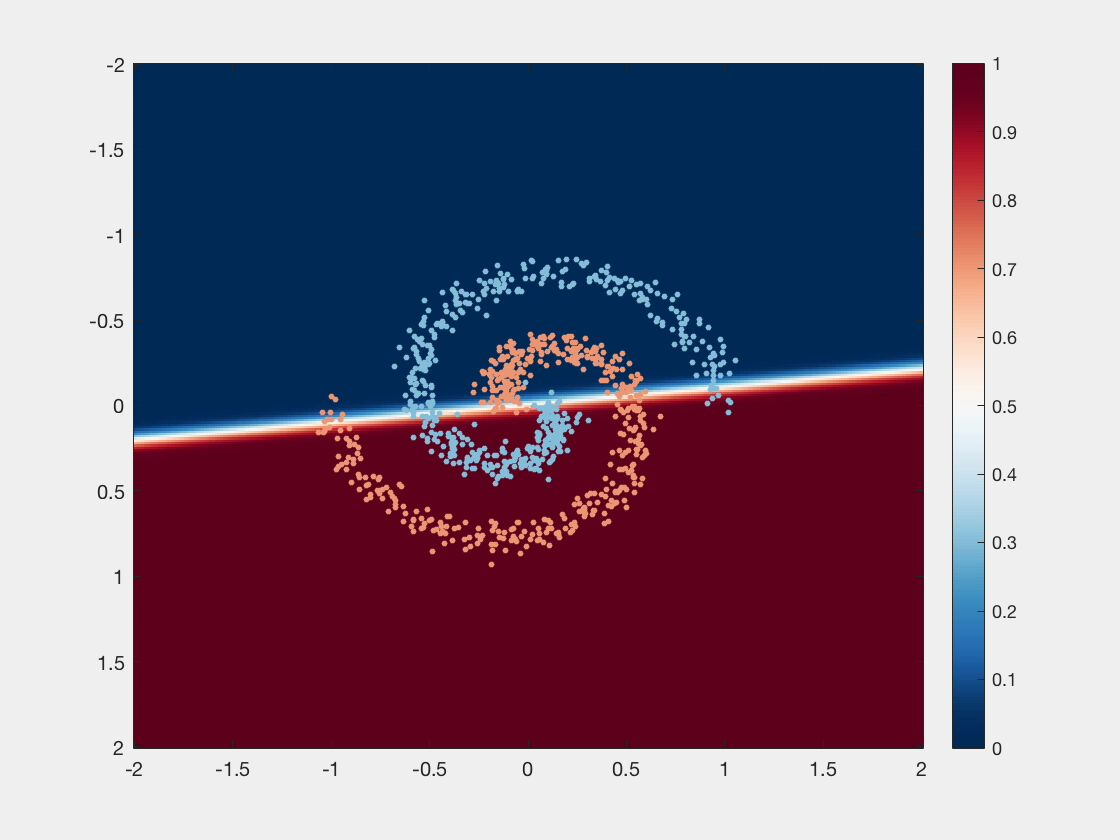
\includegraphics[width=\textwidth]{optimalcontrol/ResNet_squared_seed1_video_01}\\
            {\scriptsize $t=0$}
        \end{minipage}
        \hfill
        \begin{minipage}[b]{0.24\textwidth}
            \centering
            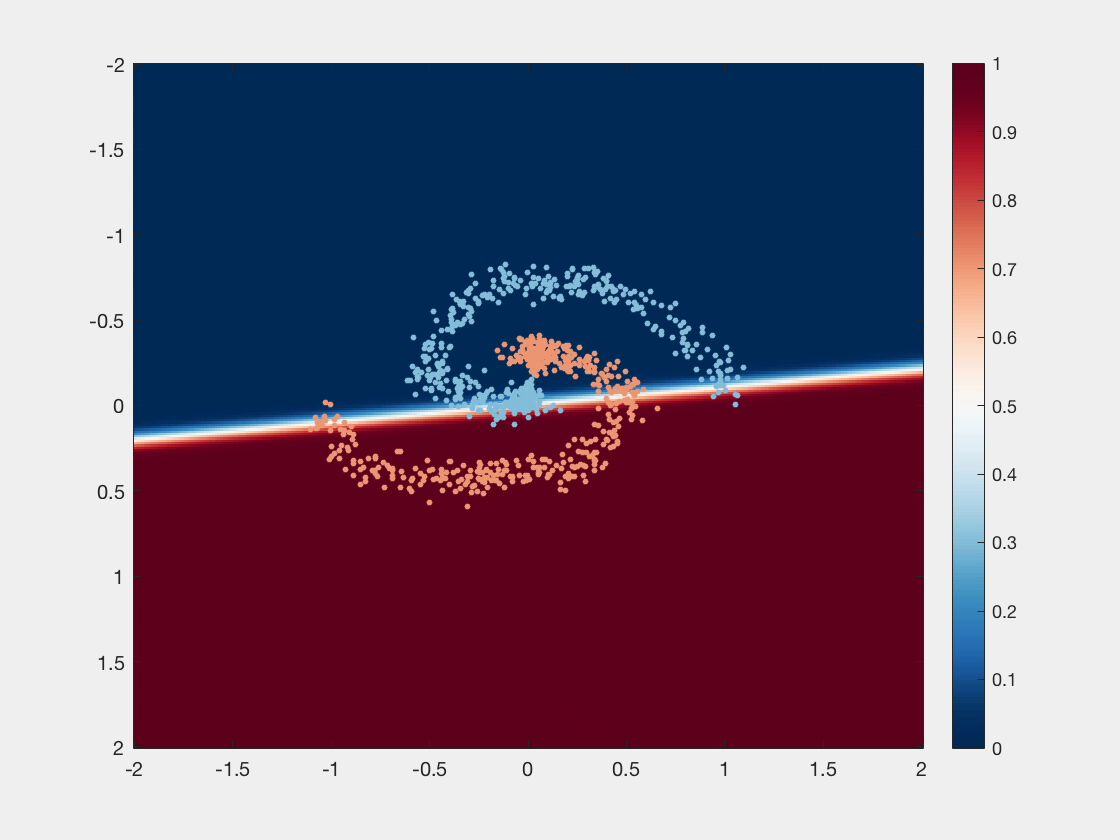
\includegraphics[width=\textwidth]{optimalcontrol/ResNet_squared_seed1_video_08}\\
            {\scriptsize $t \approx T/3$}
        \end{minipage}
        \hfill
        \begin{minipage}[b]{0.24\textwidth}
            \centering
            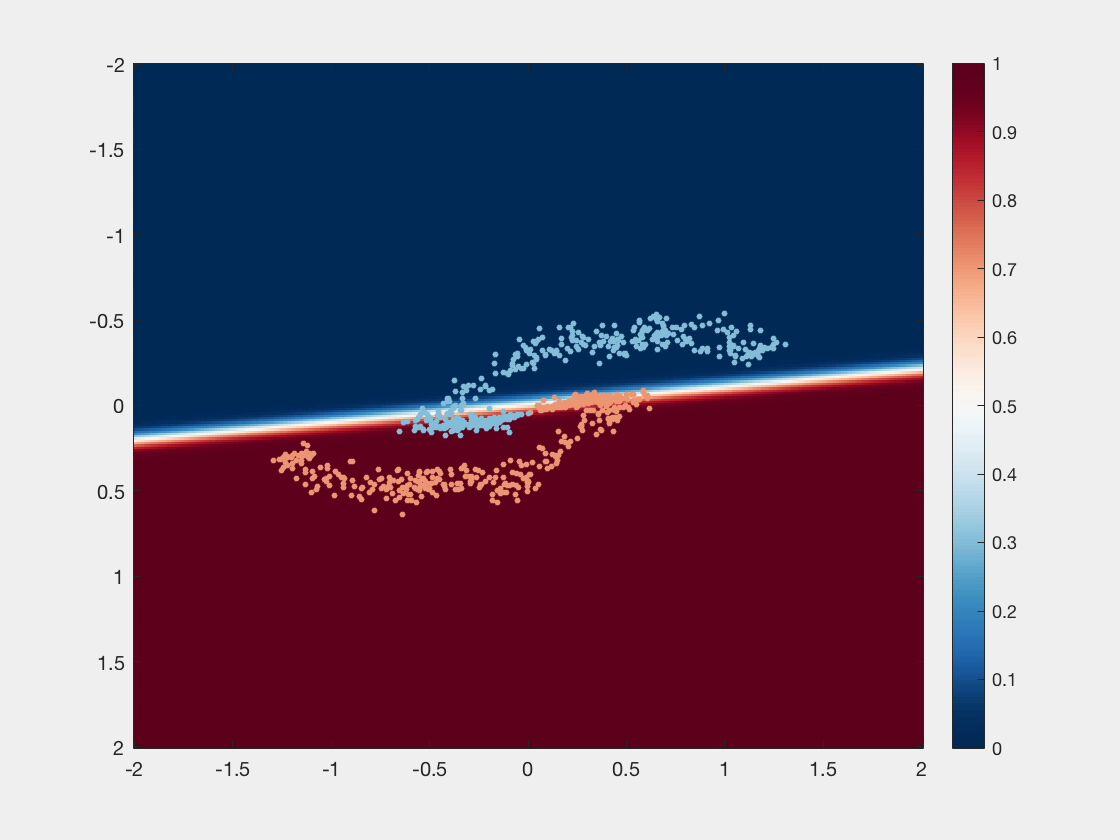
\includegraphics[width=\textwidth]{optimalcontrol/ResNet_squared_seed1_video_15}\\
            {\scriptsize $t \approx 2T/3$}
        \end{minipage}
        \hfill
        \begin{minipage}[b]{0.24\textwidth}
            \centering
            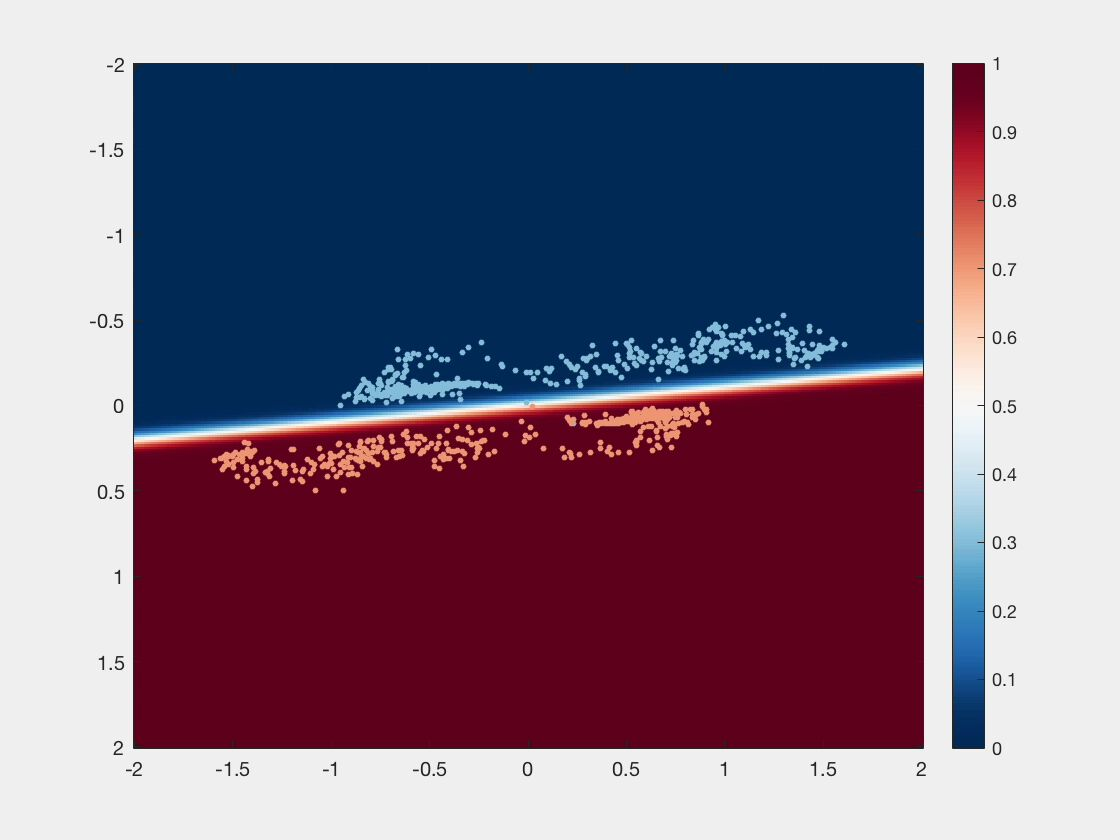
\includegraphics[width=\textwidth]{optimalcontrol/ResNet_squared_seed1_video_21}\\
            {\scriptsize $t=T$}
        \end{minipage}
        \caption{Progression of state space transformation across the continuous horizon using a ResNet flow \citep{benning2019deep}.}
    \end{figure}
\end{frame}

\begin{frame}{Connection to Monday: Discrete vs. Continuous Backprop}
    On Monday, we derived classical backpropagation by treating explicit layers as equality constraints, formulating the discrete Lagrangian yielding
    \begin{align*}
        \mathcal{L} = \mathcal{M}(x_L) + \sum_{l=1}^L \langle p_l, x_l - \sigma(W_l x_{l-1} + b_l) \rangle \, .
    \end{align*}
    Taking the gradient with respect to the state $x_l$ yielded the backward-propagating discrete adjoint equation $p_{l-1} = W_l^\top \operatorname{diag}(\sigma') p_l$.
    
    \vspace{0.5em}
    \textbf{The Continuous Generalisation:} We now apply this exact same mathematical machinery to the continuous time limit!
\end{frame}

\begin{frame}{Continuous Backpropagation: The Lagrangian}
    To perform gradient-based optimisation, we need to know how the final cost $\mathcal{J}$ reacts to continuous changes in the control signal $\Theta(t)$. 
    
    \vspace{0.5em}
    We reformulate the constrained optimal control problem into an unconstrained saddle-point problem by introducing a continuous-time Lagrange multiplier $p(t)$ (the \textbf{adjoint state}), which yields
    \begin{align*}
        \mathcal{L}(u, \Theta, p) &:= \mathcal{M}\left(u(T)\right) + \int_0^T \mathcal{R}\left(u(t), \Theta(t)\right) \, dt \\
        &\quad - \int_0^T \left\langle p(t), \frac{d}{dt}u(t) - \mathcal{F}\left(u(t), \Theta(t)\right) \right\rangle \, dt \, .
    \end{align*}
\end{frame}

\begin{frame}{Integration by Parts}
    To make it easier to take derivatives with respect to $u(t)$, we must isolate $u(t)$ from its time derivative. We apply integration by parts to the first half of the constraint integral to obtain
    \begin{align*}
        \int_0^T \left\langle p(t), \frac{d}{dt}u(t) \right\rangle dt = \langle p(T), u(T) \rangle - \langle p(0), u(0) \rangle - \int_0^T \left\langle \frac{d}{dt}p(t), u(t) \right\rangle dt \, .
    \end{align*}
    This operation elegantly shifts the time derivative from the forward state variable $u(t)$ onto the backward adjoint state $p(t)$.
\end{frame}

\begin{frame}{First-Order Optimality: The Adjoint Equation}
    By substituting this back into the Lagrangian and setting the variation with respect to the state variable $u(t)$ to zero, we obtain two coupled conditions. 
    
    \vspace{0.5em}
    At the terminal boundary $u(T)$, we observe
    \begin{align*}
        \nabla_{u(T)} \mathcal{L} = 0 \quad \implies \quad p(T) = \nabla_u \mathcal{M}\left(u(T)\right) \, .
    \end{align*}
    For the continuous interval $(0, T)$, we recover the continuous adjoint equation yielding
    \begin{align*}
        -\frac{d}{dt}p(t) = \left(\partial_u \mathcal{F}(u(t), \Theta(t))\right)^* p(t) + \nabla_u \mathcal{R}(u(t), \Theta(t)) \, .
    \end{align*}
    \pause
    Notice that the adjoint state evolves \textbf{backwards in time}. This is the strict continuous-time analogue of discrete backpropagation.
\end{frame}

\begin{frame}{First-Order Optimality: The Control Gradient}
    Finally, taking the variation with respect to the continuous control parameters $\Theta(t)$ isolates the exact gradient we need for learning yielding
    \begin{align*}
        \nabla_{\Theta(t)} \mathcal{L} = \left(\partial_\Theta \mathcal{F}(u(t), \Theta(t))\right)^* p(t) + \nabla_\Theta \mathcal{R}\left(u(t), \Theta(t)\right) = 0 \, .
    \end{align*}\pause
    
    \vspace{0.5em}
    During gradient-based training, if we have not yet converged to the optimal parameters, the left-hand side of this equation directly supplies the continuous gradient $\nabla_{\Theta(t)} \mathcal{J}$ required to equivalently update $\Theta(t)$.
\end{frame}

\begin{frame}{The Hamiltonian \& Pontryagin's Minimum Principle}
    We can encapsulate the required equations in a single functional called the \textbf{Hamiltonian}, $\mathcal{H}$:
    \begin{align*}
        \mathcal{H}\left(u(t), p(t), \Theta(t)\right) := \left\langle p(t), \mathcal{F}\left(u(t), \Theta(t)\right) \right\rangle + \mathcal{R}\left(u(t), \Theta(t)\right) \, .
    \end{align*}
    By computing the partial derivatives of the Hamiltonian, we recover the foundational set of continuous optimality conditions, i.e.,
    \begin{align*}
        \frac{d}{dt} u(t) &= \nabla_p \mathcal{H} \quad (\text{State Equation}) \\
        -\frac{d}{dt} p(t) &= \nabla_u \mathcal{H} \quad (\text{Adjoint Equation}) \\
        0 &= \nabla_\Theta \mathcal{H} \quad (\text{Optimality Condition}) 
    \end{align*}
    This theoretical architecture forms the backbone of \textbf{Pontryagin's Minimum Principle}.
\end{frame}

%================================================================%
\section{Discretisation and Architectural Design}
%================================================================%

\begin{frame}{Evaluating Continuous Control Computationally}
    There are two competing paradigms in numerical optimal control for deep learning:
    
    \vspace{0.5em}
    \begin{enumerate}
        \item \textbf{First-discretise-then-optimise:} Standard deep learning. Discretise the continuous flow into fixed layers, then calculate discrete gradients via backpropagation.
        \item \textbf{First-optimise-then-discretise:} Derive the continuous adjoint equations first (as we just did), and \emph{then} discretise the resulting two-point boundary value problem using numerical ODE solvers.
    \end{enumerate}
\end{frame}

\begin{frame}{Beyond Forward Euler: Runge-Kutta Methods}
    While standard ResNets implicitly use Forward Euler, this is a first-order method requiring exceptionally small time steps (and thus very deep networks) for stability. By adopting \textbf{Runge-Kutta (RK)} methods, we achieve higher-order approximations.
    
    \vspace{0.5em}
    A generic $s$-stage RK scheme for the forward state equation computes the next state via intermediate stages $U_i$:
    \begin{align*}
        U_i^l &= u^l + \Delta t \sum_{j=1}^s a_{i,j} \mathcal{F}(U_j^l, \Theta_j^l) \, , \\
        u^{l+1} &= u^l + \Delta t \sum_{i=1}^s b_i \mathcal{F}(U_i^l, \Theta_i^l) \, .
    \end{align*}
\end{frame}

\begin{frame}{The Partitioned Runge-Kutta (PRK) Method}
    Deep learning requires solving a coupled two-point boundary value problem: integrating the state $u(t)$ forward in time, and integrating the adjoint $p(t)$ backward in time.
    
    \vspace{0.5em}
    To handle this, we employ a \textbf{Partitioned Runge-Kutta (PRK)} method. This applies one RK scheme to the forward equation, and a distinct, mathematically matched RK scheme (with weights $\tilde{b}_i$ and matrix $\tilde{a}_{i,j}$) to the backward adjoint equation yielding
    \begin{align*}
        P_i^l &= p^l + \Delta t \sum_{j=1}^s \tilde{a}_{i,j} \ell_j^l \, , \\
        p^{l+1} &= p^l + \Delta t \sum_{i=1}^s \tilde{b}_i \ell_i^l \, .
    \end{align*}
\end{frame}

\begin{frame}{Symplectic Discretisation}
    \pause
    \begin{theoremblock}{Symplectic Discretisation}
        The "first-discretise" and "first-optimise" approaches \textbf{perfectly commute} (yielding the exact same gradients) only if the chosen discretisation scheme is a \textbf{Symplectic Partitioned Runge-Kutta (PRK)} method \citep{hager2000runge}.
    \end{theoremblock}
    
    \vspace{0.5em}
    For a PRK to be symplectic, it must perfectly preserve the discrete inner product $\langle p^{l+1}, v^{l+1} \rangle = \langle p^l, v^l \rangle$. This algebraically requires
    \begin{align*}
        b_i = \tilde{b}_i \quad \text{and} \quad b_i\tilde{a}_{i,j} + \tilde{b}_j a_{i,j} - b_i\tilde{b}_j = 0 \quad \text{for all } i, j \, .
    \end{align*}
\end{frame}

\begin{frame}{Example: The Symplectic Euler Method}
    Consider the simplest symplectic PRK. Rather than using forward Euler for both passes, we pair the \emph{explicit} Euler for the state with the \emph{implicit} Euler for the adjoint.
    
    \vspace{0.5em}
    For a single stage ($s=1$), the forward explicitly uses $b_1 = 1, a_{1,1} = 0$. By the symplectic conditions, we must have
    \begin{itemize}
        \item $\tilde{b}_1 = b_1 = 1$.
        \item $1 \cdot \tilde{a}_{1,1} + 1 \cdot 0 - 1 \cdot 1 = 0 \implies \tilde{a}_{1,1} = 1$ (Implicit Euler).
    \end{itemize}
    
    \vspace{0.5em}
    This pairing precisely forms the backbone of standard ResNet backpropagation, natively preserving discrete Hamiltonian dynamics!
\end{frame}

\begin{frame}{ODENets \& Learnable Time Steps}
    When treating deep learning as an ODE, the "time step" $\Delta t$ between layers does not necessarily need to be a fixed hyperparameter but can become a \textbf{learnable parameter} $\alpha$.\pause
    
    \vspace{0.5em}
    In the ODENet architecture, the control set is expanded to $\Theta = (W, \beta, \alpha)$, allowing the network to dynamically adjust the integration step size.\pause 
    
    \vspace{0.5em}
    \textbf{Simplex Constraints:} We can force extreme sparsity by projecting these learnable time steps onto a probability simplex $\mathcal{S} = \{ \alpha \mid \alpha \ge 0, \sum \alpha = 1 \}$. The network automatically sets most time steps to exactly zero, compressing the depth dynamically during inference.
\end{frame}

\begin{frame}{Empirical Results: ODENets}
    When the simplex constraint is applied, the network drops unnecessary steps. This compresses a deep 20-layer network down to just 2 or 3 active layers.
    
    \begin{figure}[htpb]
        \centering
        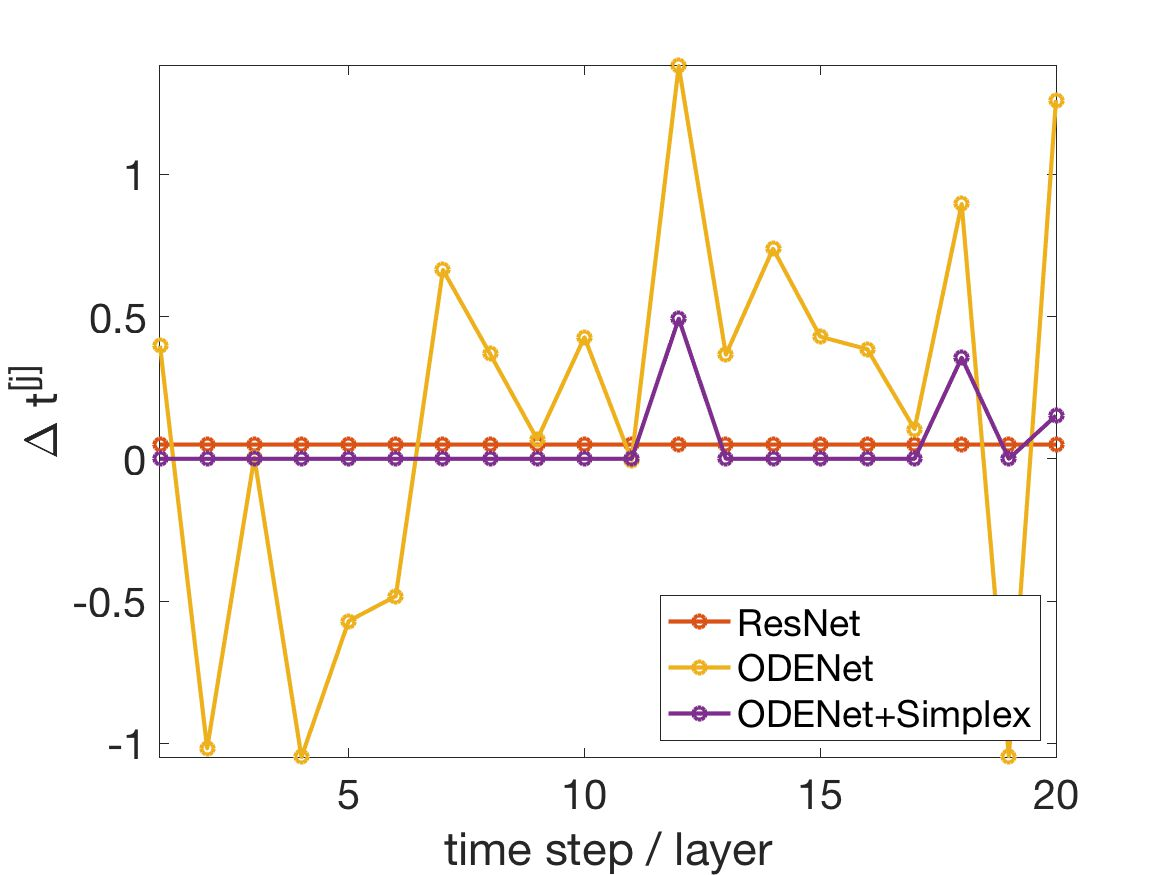
\includegraphics[width=0.375\textwidth]{optimalcontrol/example_squares2d_20layers_backtracking1_seed1_timesteps}
        \caption{Learned time steps for ResNet, ODENet, and ODENet+Simplex \citep{benning2019deep}.}
    \end{figure}
\end{frame}

\begin{frame}{Variational Networks (VNs): Reversing the Perspective}
    Instead of analysing an artificial neural network as an ODE, we can \emph{derive} neural networks directly by discretising the continuous gradient flows of established physical energy functionals.
    
    \vspace{0.5em}
    Using a highly parameterised \textbf{Fields of Experts (FoE)} regulariser \citep{roth2005fields}, we define the continuous energy yielding
    \begin{align*}
        E(u) = \frac{\lambda}{2} \|K u - f^\delta\|_2^2 + \sum_{i=1}^{N_D} \sum_{p} \rho_i\left((D_i u)_p\right) \, .
    \end{align*}
    Here, $K$ is the physics forward operator, $D_i$ are learned convolutional filters, and $\rho_i$ are learned non-linear RBF potentials.
\end{frame}

\begin{frame}{Incremental Gradient Steps (Unrolling)}
    By unrolling the continuous gradient descent of this specific functional, we naturally arrive at the powerful \textbf{Variational Network (VN)} architecture \citep{hammernik2018learning}.
    
    \vspace{0.5em}
    Calculating the derivative with respect to $u$ and formulating a discrete step yields
    \begin{align*}
        u^{t+1} = u^t - \left( \sum_{i=1}^{N_D} (D_i^t)^\top \rho_i^{t\prime}(D_i^t u^t) + \lambda^t K^*(K u^t - f^\delta) \right) \, .
    \end{align*}
    This exactly mirrors the computational architecture of deep ResNets, where the data fidelity acts as a skip connection enforcing physical consistency.
\end{frame}

\begin{frame}{Variational Network Architecture}
    This architecture fuses rigorous theoretical physics with parameterised expressiveness.
    
    \begin{figure}[htpb]
        \centering
        \begin{minipage}[t]{0.48\textwidth}
            \centering
            % Bottom half: trim more from top (use 0 <height> 0 0 in bp)
            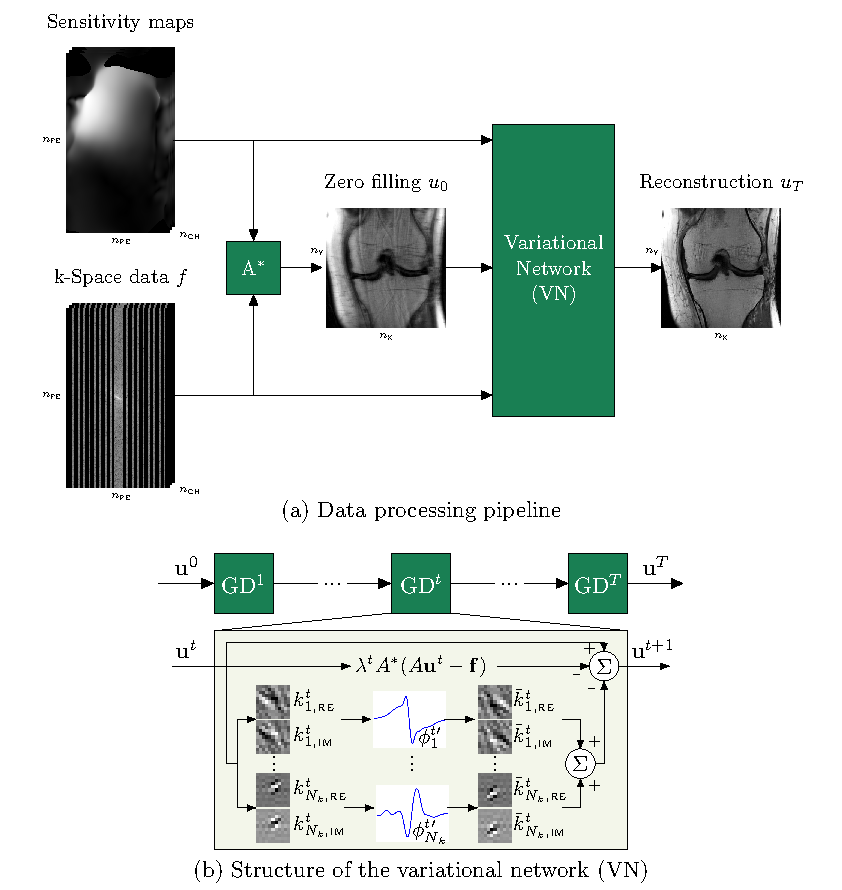
\includegraphics[width=\textwidth,clip,trim=0 190bp 0 0]{varnetworks/figure1-vn_overview}
        \end{minipage}\hfill
        \begin{minipage}[t]{0.48\textwidth}
            \centering
            % Top half: trim more from bottom (use 0 0 0 <height> in bp)
            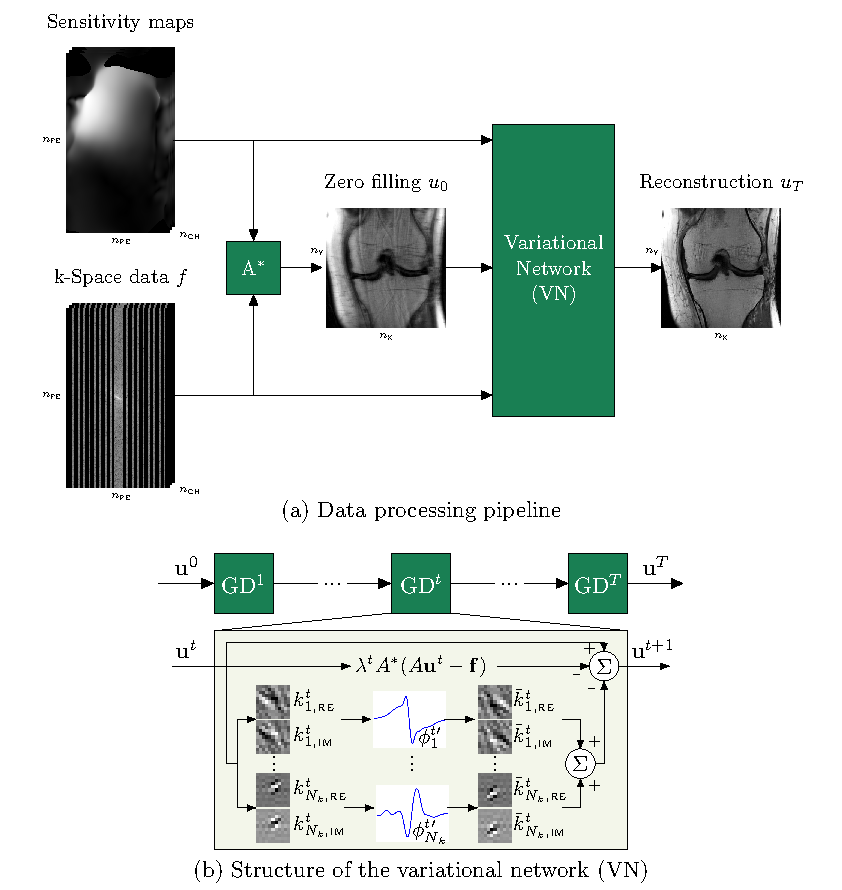
\includegraphics[width=\textwidth,clip,trim=0 0 0 250bp]{varnetworks/figure1-vn_overview}
        \end{minipage}
        
        \vspace{0.5em}
        \caption{Overview of a Variational Network architecture simulating an unrolled energy minimisation \citep{hammernik2018learning}.}
    \end{figure}
\end{frame}

\begin{frame}{Convex vs. Non-Convex Limits}
    A profound theoretical advantage of VNs is the ability to easily constrain the network to be strictly convex. By restricting the RBF weights to be positive and applying zero-mean constraints to the filters $D_i$, the energy landscape becomes globally convex.
    
    \vspace{0.5em}
    \textbf{The Tradeoff:} 
    Convex models provide theoretical guarantees, but fundamentally penalise large gradients too aggressively, degrading images. Highly parameterised non-convex VNs consistently outperform them empirically on in-distribution examples by capturing complex, high-frequency textures \citep{kobler2017variational}.
\end{frame}

\begin{frame}{Application to Clinical MRI}
    When applied to accelerated MRI, the network maps the complex signal into an embedded real-valued domain $\mathbb{R}^{2N}$, calculating dense filter responses for both the real and complex planes.
    
    \vspace{0.5em}
    To train these complex-to-real models over a dataset of undersampled clinical measurements $f_s^\delta$ and fully sampled references $u_s$, the loss function combines a robust $L_1$ norm with a complex-valued Structural Similarity Index (SSIM) yielding
    \begin{align*}
        \min_{\Theta} \sum_{s=1}^S \left( \| u_s - u_T(\Theta, f_s^\delta) \|_1 + \gamma \mathcal{L}_{\text{SSIM}}(u_s, u_T(\Theta, f_s^\delta)) \right) \, .
    \end{align*}
\end{frame}

\begin{frame}{Interpreting Learned Filters}
    Because the unrolled layers are strictly structured as a trainable Field of Experts model, reading the trained network's explicit linear filters reveals easily recognizable motifs (e.g., directional Gabor-like filters and finite-difference operators).
    
    \begin{figure}[htpb]
        \centering
        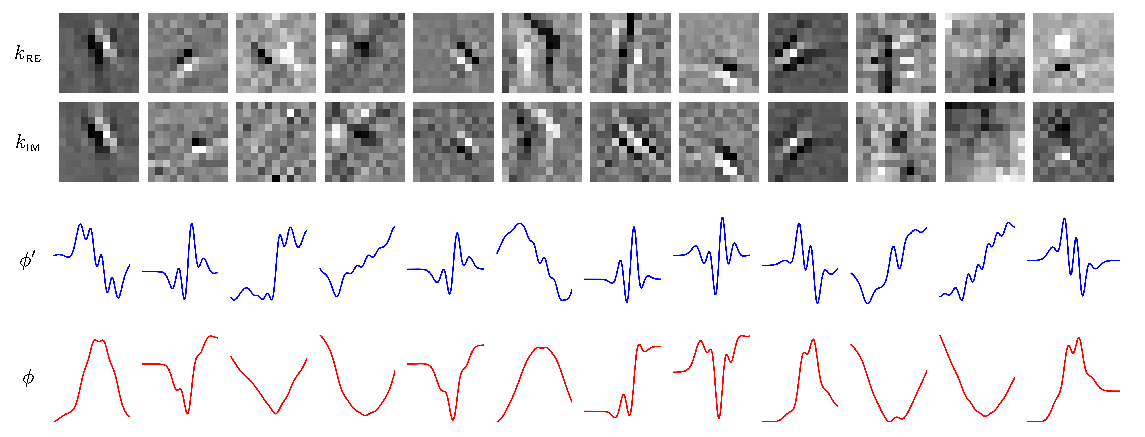
\includegraphics[width=0.7\textwidth]{varnetworks/figure9-parameters}
        \caption{Visualisation of the learned convolutional filters $D_i$ \citep{hammernik2018learning}.}
    \end{figure}
\end{frame}

\begin{frame}{Robust Generalisation to Unseen Pathologies}
    Because the network enforces the physical forward operator $K$ continuously, it avoids the aggressive hallucination phenomena commonly crippling pure black-box CNNs.
    
    \begin{figure}[htpb]
        \centering
        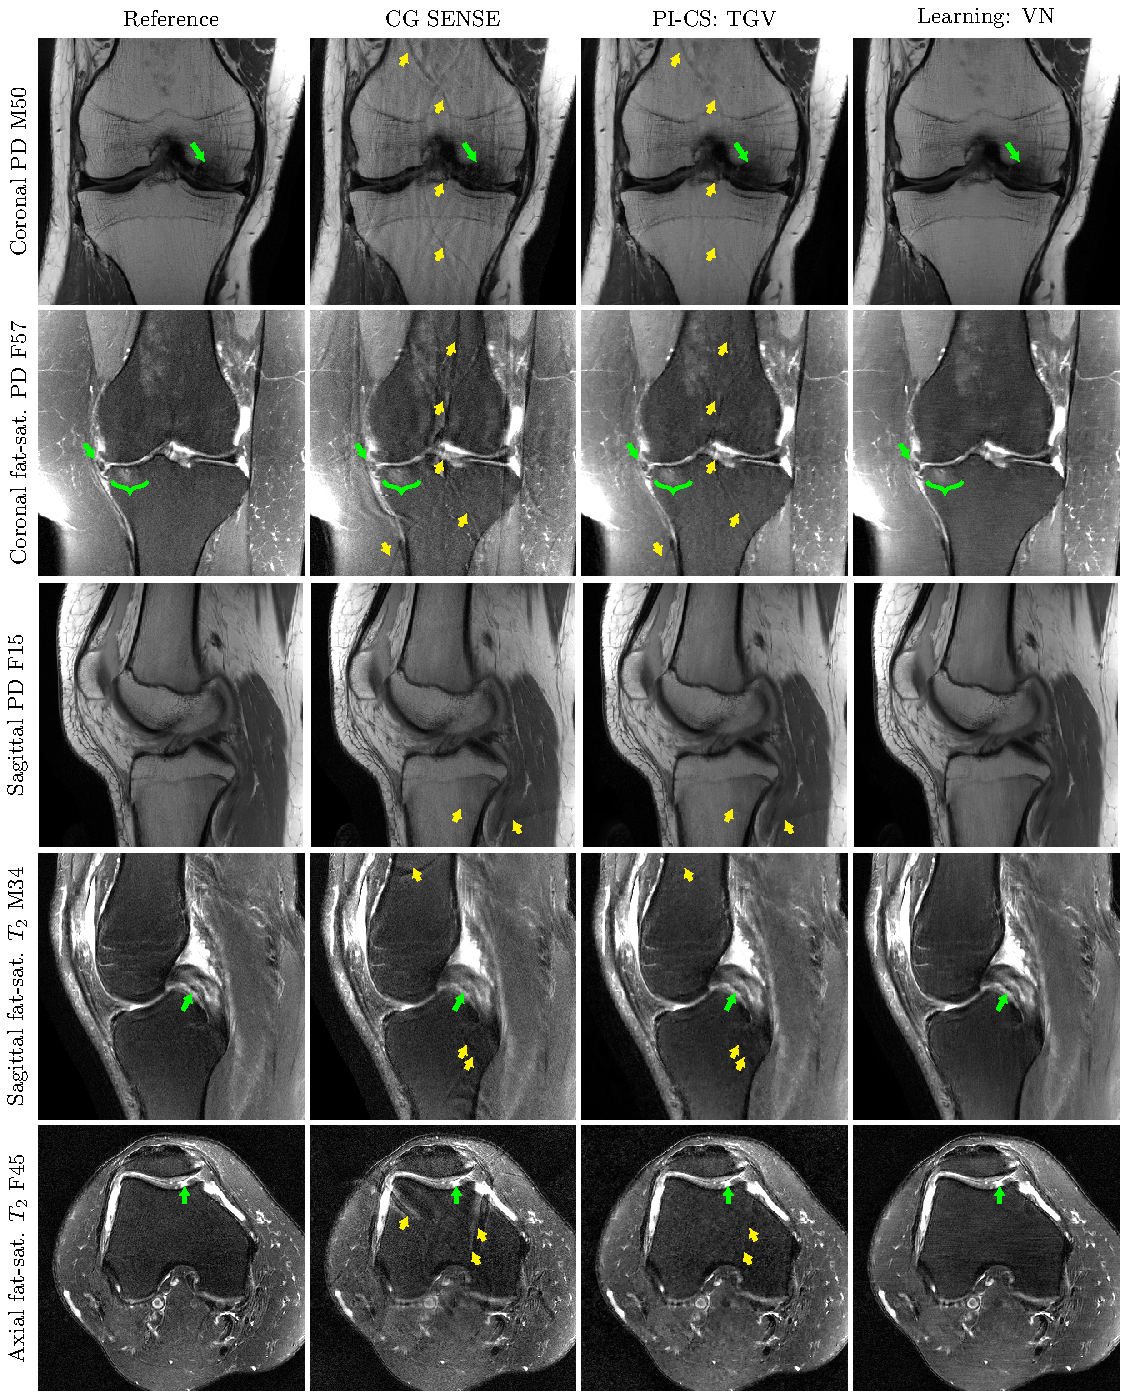
\includegraphics[width=0.7\textwidth]{varnetworks/figure7-result_kneeprotocol}
        \caption{Despite never having seen a specific meniscal tear during training, the VN successfully reconstructs the exact unseen pathology \citep{hammernik2018learning}.}
    \end{figure}
\end{frame}

%================================================================%
\section{The Early Stopping Paradox \& Dynamic Depth}
%================================================================%

\begin{frame}{The Early Stopping Paradox}
    In classical variational image processing and modern unrolled networks, a counter-intuitive phenomenon emerges.
    
    \vspace{0.5em}
    \begin{alertblock}{The Paradox}
        Strictly converging to the global minimum of the regularised continuous energy functional $E(u)$ often yields \textbf{worse} image quality than stopping the iterative minimisation algorithm early!
    \end{alertblock}
    
    \pause
    \vspace{0.5em}
    This occurs because even highly expressive data-driven priors cannot perfectly model the true, infinite-dimensional manifold of natural images. As iterations $t \to \infty$, modelling errors compound and destroy structural image textures (e.g., TV-$L^2$ staircasing).
\end{frame}

\begin{frame}{Visualising the Paradox}
    Optimal visual and mathematical fidelity peaks at intermediate iterations. Further continuous gradient steps actively degrade the image. Finite halting depth is structurally necessary.
    
    \begin{figure}[htpb]
        \centering
        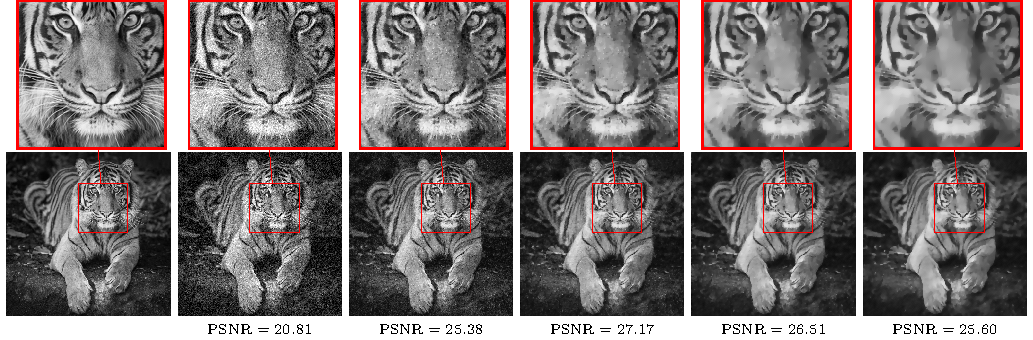
\includegraphics[width=0.85\textwidth]{varnetworks/fig2}
        \caption{The Early Stopping Paradox. Images after 13, 26, 39, and 52 iterations. Fidelity peaks at 26 iterations \citep{effland2020variational}.}
    \end{figure}
\end{frame}

\begin{frame}{Stopping Time as a Control Parameter}
    How do we determine this stopping point rigorously, rather than relying on arbitrary hyperparameters? 
    
    \vspace{0.5em}
    By formulating VNs as a continuous optimal control problem, we can make the stopping time $T$ a \textbf{continuously learnable parameter}. We employ time-reparameterisation $x(t) = u(tT)$ to map the bounds to exactly $t \in (0, 1)$. The state ODE becomes
    \begin{align*}
        \frac{d}{dt}x(t) = T \mathcal{F}(x(t), \Theta) \, .
    \end{align*}
    Notice that $T$ acts as a scalar multiplier scaling the entire continuous velocity vector field!
\end{frame}

\begin{frame}{Optimality Conditions for Network Depth}
    By evaluating the variation of the Lagrangian strictly with respect to the scalar horizon $T$, we recover a rigorous first-order necessary condition yielding
    \begin{align*}
        \int_0^1 \left\langle p(t), \frac{d}{dt}x(t) \right\rangle \, dt = 0 \, .
    \end{align*}
    
    \vspace{0.5em}
    This elegantly states that at the continuous global minimum of stopping time $T$, the network's forward ODE velocity and the adjoint error gradient field must be perfectly \textbf{structurally orthogonal} \citep{effland2020variational}.
\end{frame}

\begin{frame}{Nonlinear Spectral Dynamics}
    Why does the continuous flow improve the image before destroying it? 
    
    \vspace{0.5em}
    If we perform an eigenvalue decomposition of the continuous field-of-experts gradients, we reveal exactly what the discretised layers dynamically evaluate:
    
    \begin{itemize}
        \item \textbf{High-frequency, noisy scatter patterns:} Produce huge eigenvalues. The network applies massive damping, rapidly annihilating noise in the first few layers.
        \item \textbf{Structural boundaries and textures:} Produce eigenvalues near zero. The contraction factor is $\approx 1$, meaning structures are only smoothed extremely slowly over time.
    \end{itemize}
    \vspace{0.5em}
    The unrolled network acts as a nonlinear dynamic spectral filter, and learning $T$ halts the flow perfectly before macro-structures degrade.
\end{frame}

\begin{frame}{Eigenpairs in Action}
    \begin{figure}[htpb]
        \centering
        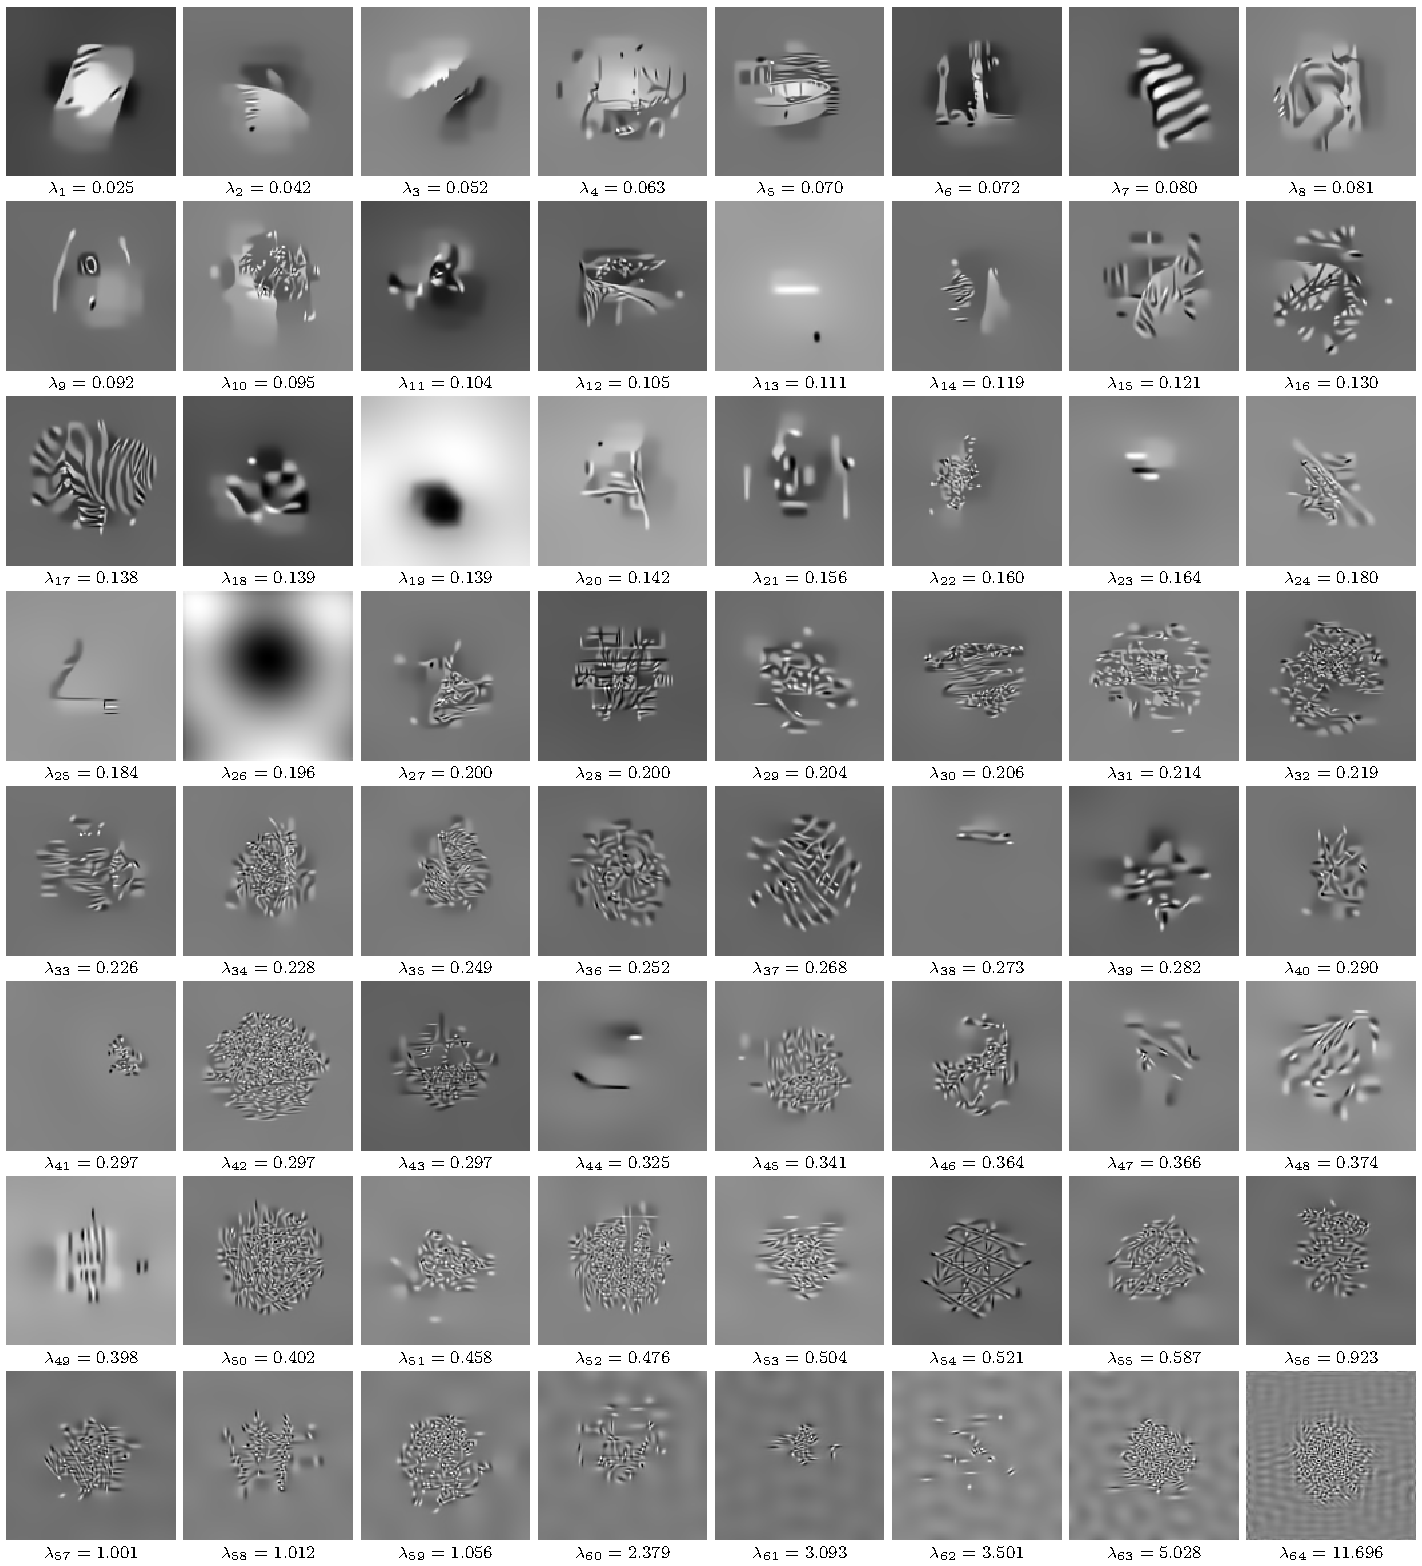
\includegraphics[width=0.85\textwidth]{varnetworks/fig13}
        \caption{Computed general eigenpairs. Lower eigenvalue coefficients $\lambda$ match large-scale structures and tissue boundaries, shielding them organically from strong attenuation \citep{effland2020variational}.}
    \end{figure}
\end{frame}

%================================================================%
\section{Implicit Deep Learning \& Deep Equilibrium Models (DEQ)}
%================================================================%

\begin{frame}{The Limits of Finite Depth}
    Whether we unroll $L$ discrete layers or solve an ODE up to time $T$, we are still bound by a forward trajectory that must be stored in memory for continuous backpropagation.
    
    \vspace{0.5em}
    \begin{alertblock}{The Truncation Error Problem}
        Utilising a fixed, pre-determined number of layers $L$ restricts flexibility. If an unrolled model requires more iterations to converge at inference time than it was trained for, it often suffers from severe truncation errors and mathematical instability \citep{gilton2021deep}.
    \end{alertblock}
\end{frame}

\begin{frame}{Visualising the Memory Footprint}
    \begin{figure}[htpb]
        \centering
        \begin{minipage}{0.33\textwidth}
            \centering
            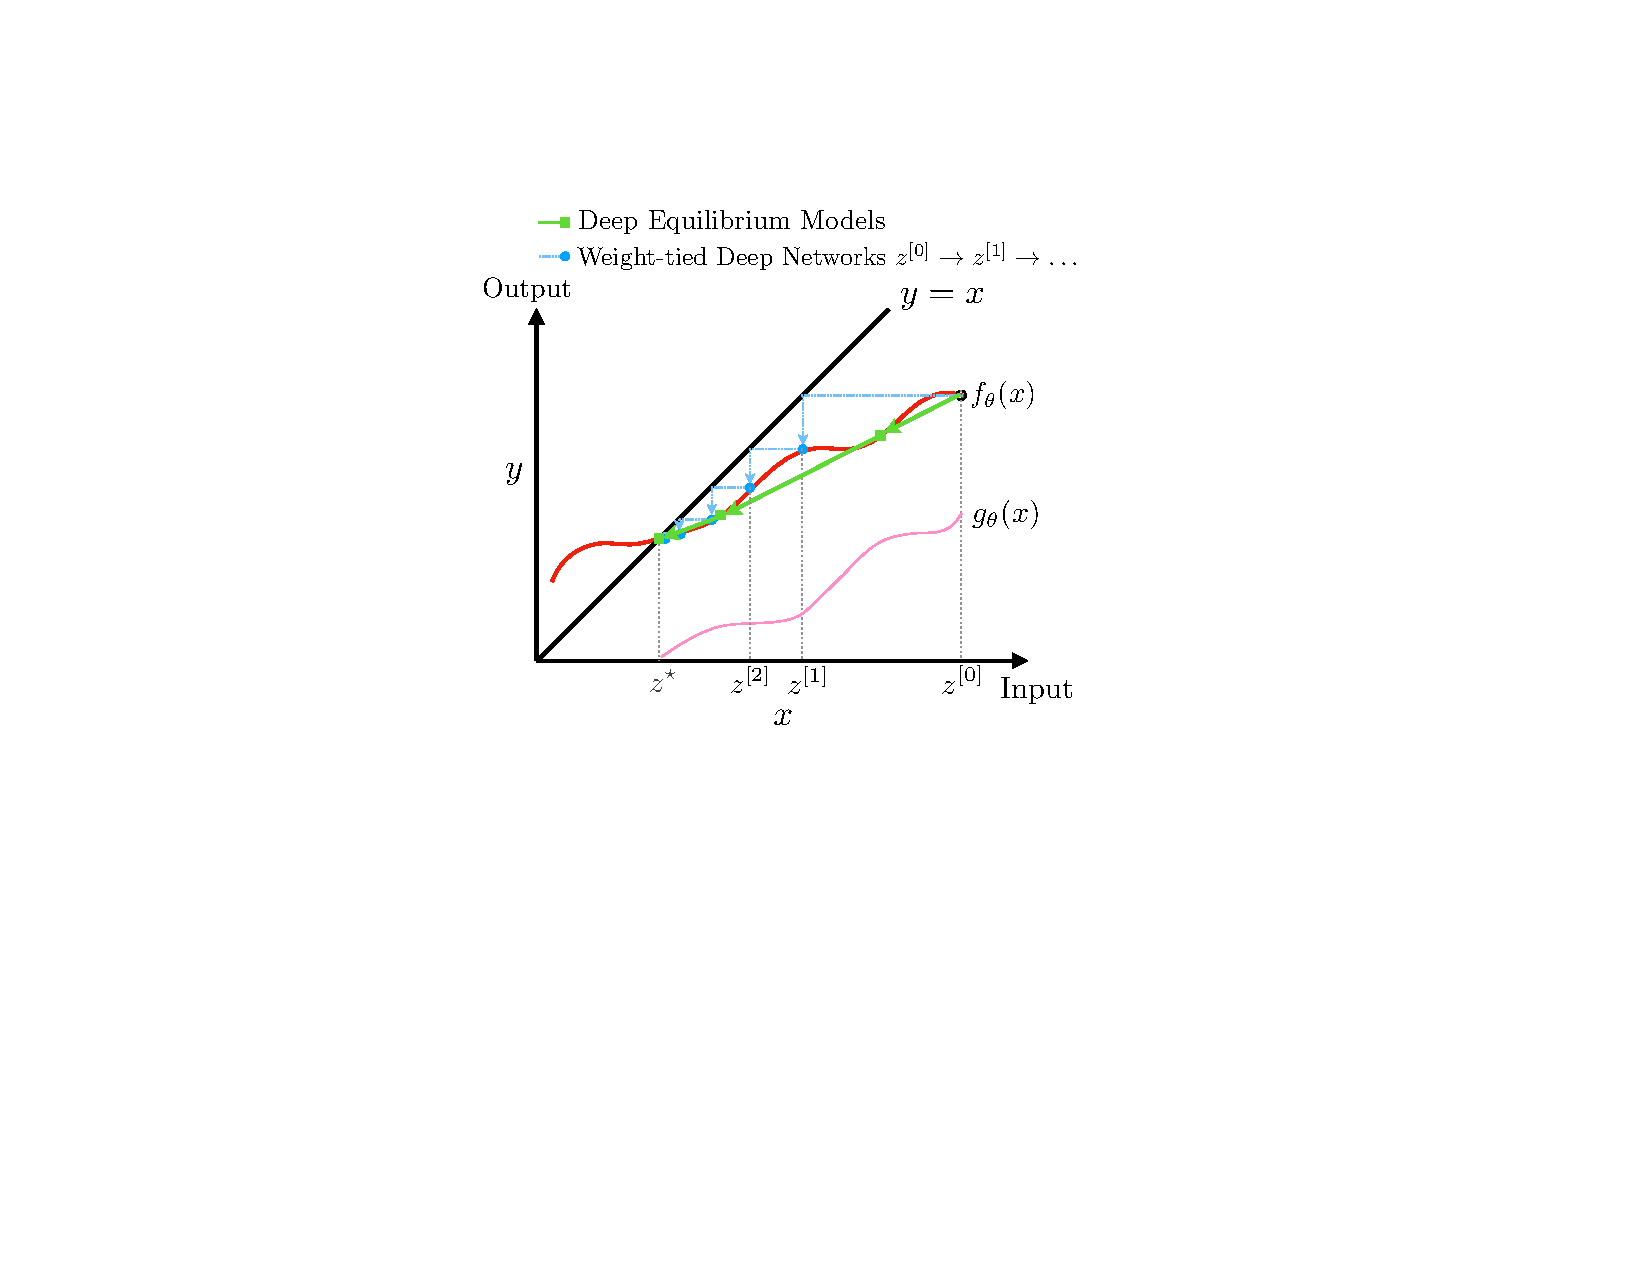
\includegraphics[width=\textwidth]{deq/fp_onefig}\\
            {\scriptsize Solving for an equilibrium point in 2D.}
        \end{minipage}
        \hfill
        \begin{minipage}{0.6\textwidth}
            \centering
            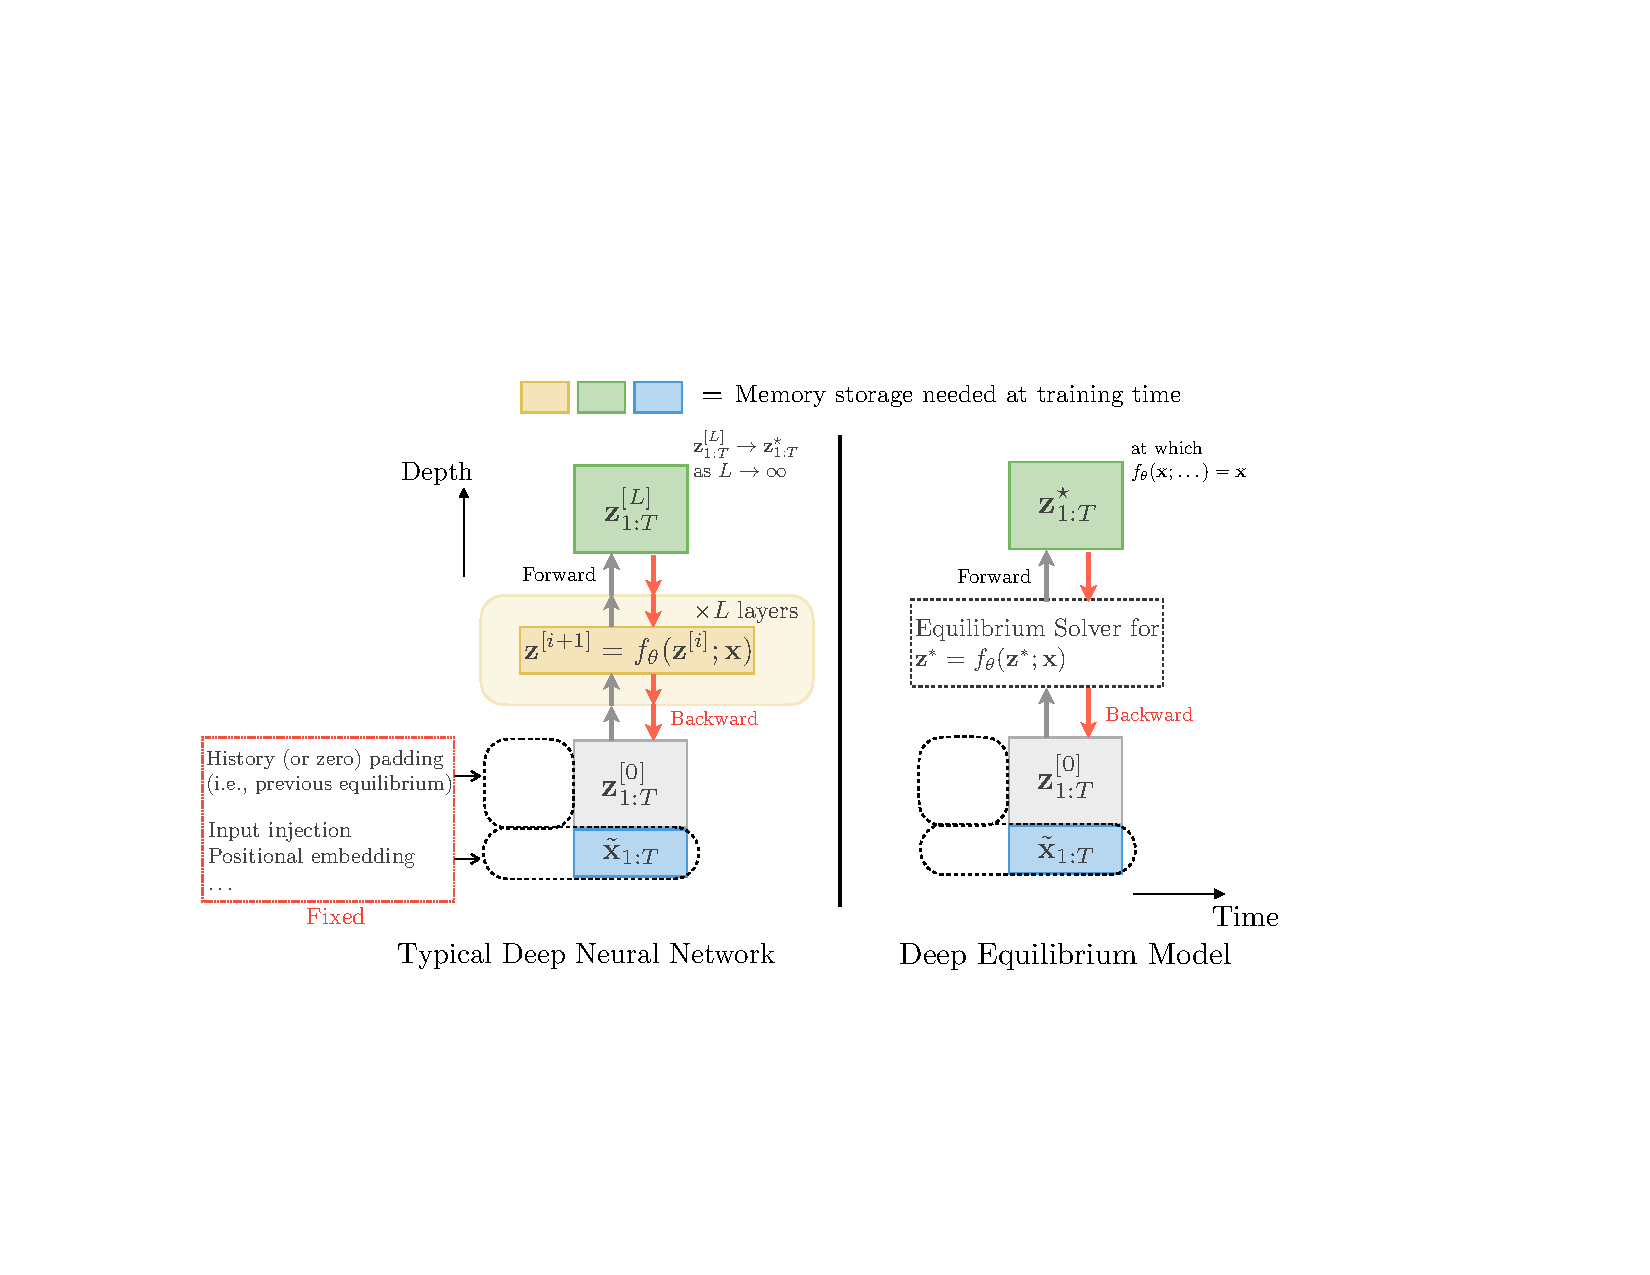
\includegraphics[width=\textwidth]{deq/equm_vs_dnn}\\
            {\scriptsize DEQ vs conventional deep network memory.}
        \end{minipage}
        \caption{Explicit layer stacking requires storing intermediate activations, yielding memory growth with depth. DEQs compute an equilibrium state with constant memory usage \citep{bai2019deep}.}
    \end{figure}
\end{frame}

\begin{frame}{The Paradigm Shift: Implicit Models}
    \begin{theoremblock}{Deep Equilibrium Models (DEQs)}
        DEQs \citep{bai2019deep} bypass trajectories entirely. Instead of explicitly tracking depth, we define the output of the network purely as the steady-state \textbf{equilibrium condition} of a weight-tied mapping:
        \begin{align*}
            z^\star = f_\theta(z^\star, x) \, .
        \end{align*}
    \end{theoremblock}
    Here, $x$ is the input, $z^\star$ is the hidden state output, and $f_\theta$ is the core transformation block. Rather than a side effect of a finite algorithm, the fixed point becomes the central object.
\end{frame}

\begin{frame}{Universality of Equilibrium Layers}
    Does replacing explicit depth with a single implicit equilibrium condition reduce expressivity? 
    
    \vspace{0.5em}
    \textbf{No.} The DEQ perspective separates \emph{how} a representation is computed from \emph{what} representation is admissible at equilibrium.
    
    \vspace{0.5em}
    \begin{itemize}
        \item \textbf{Universality:} A single implicit DEQ layer on an augmented hidden state is as expressive as any infinitely deep explicit network.
        \item \textbf{Stacking is Redundant:} Any finite stack of DEQ blocks can be mathematically rewritten as one large DEQ block. Macroscopic stacking provides absolutely no additional representational power.
    \end{itemize}
\end{frame}

\begin{frame}{The Forward Pass: Root-Finding}
    Because the output is simply the equilibrium point, the forward pass Abandons layer-by-layer execution. We recast the fixed-point condition as a root-finding problem yielding
    \begin{align*}
        g_\theta(z^\star, x) := f_\theta(z^\star, x) - z^\star = 0 \, .
    \end{align*}
    
    \pause
    \vspace{0.5em}
    To solve this, basic fixed-point (Picard) iteration $z_{k+1} = f_\theta(z_k, x)$ provides guarantees for strict contractions but is unacceptably slow. DEQs use accelerated black-box solvers instead.
\end{frame}

\begin{frame}{Broyden's Method}
    Newton's method leverages first-order derivative information via the Jacobian matrix $J_{g_\theta}$, but explicitly inverting the massive $d \times d$ Jacobian matrix is computationally infeasible.
    
    \vspace{0.5em}
    \textbf{Broyden's Method} circumvents this by acting as a quasi-Newton method, replacing the exact inverse Jacobian with an iterative approximation $H_k \approx J_{g_\theta}(z_k, x)^{-1}$. The update modifies $H_k$ using a \textbf{rank-one update} yielding
    \begin{align*}
        H_k = H_{k-1} + \frac{(\Delta z_k - H_{k-1}\Delta g_k)\,\Delta g_k^\top}{\|\Delta g_k\|_2^2} \, .
    \end{align*}
\end{frame}

\begin{frame}{Anderson Acceleration (AA)}
    Instead of Newton updates, Anderson Acceleration forms an affine combination of recent iterates that minimises the current residual in a small least-squares problem \citep{walker2011anderson}.
    
    \vspace{0.5em}
    \textbf{The Connection:} AA exposes an algebraic link to multisecant quasi-Newton updates. Furthermore, when applied to a strictly linear system, Anderson Acceleration becomes mathematically equivalent to the \textbf{Generalised Minimal Residual method (GMRES)}, a highly robust iterative solver crucial for our backward pass!
\end{frame}

\begin{frame}{The Backward Pass: Implicit Differentiation}
    How do we compute gradients for backpropagation without unrolling the root-finding solver and hitting the $\mathcal{O}(L)$ memory bottleneck?
    
    \vspace{0.5em}
    We use \textbf{Implicit Differentiation}! As we derived on Tuesday for Bilevel hyperparameter learning, we formulate the backward pass as a constrained optimisation problem. We want to minimise an empirical risk loss objective $\mathcal{L}_{\text{task}}$ constrained by the equilibrium condition.
    
    \vspace{0.5em}
    The Lagrangian formulation reads
    \begin{align*}
        \mathcal{L}(z, \theta; v) = \mathcal{L}_{\text{task}}(z, \theta) - \langle v, z - f_\theta(z; x) \rangle \, .
    \end{align*}
\end{frame}

\begin{frame}{The Adjoint Fixed-Point Equation}
    Applying the Karush-Kuhn-Tucker (KKT) conditions, we set the gradient of the Lagrangian with respect to the state $z$ to zero. This derives the exact, steady-state adjoint equation yielding
    \begin{align*}
        v = J_{f_\theta}^{\top} v + \nabla_z \mathcal{L}_{\text{task}}(z^\star, \theta) \, ,
    \end{align*}
    where $J_{f_\theta}^{\top}$ is the transposed Jacobian of the forward cell.
    
    \vspace{0.5em}
    \begin{alertblock}{$\mathcal{O}(1)$ Memory Training}
        Because we compute the adjoint variable $v$ using a linear solver directly at the equilibrium point $z^\star$, we completely discard the intermediate forward trajectory. Training requires \textbf{strictly constant memory $\mathcal{O}(1)$}, regardless of effective depth!
    \end{alertblock}
\end{frame}

\begin{frame}{Convergence Guarantees: Spectral Symmetry}
    A remarkable mathematical synergy arises when guaranteeing convergence for both the forward and backward passes.
    
    \vspace{0.5em}
    Because the linear operator driving the adjoint iteration is explicitly $J_{f_\theta}^{\top}$, it shares exactly the same eigenvalues as the forward Jacobian $J_{f_\theta}$. Thus, their spectral radii remain identical:
    \begin{align*}
        \rho(J_{f_\theta}^{\top}) = \rho(J_{f_\theta}) \, .
    \end{align*}
    Therefore, if the forward pass converges as a strict contraction mapping, the adjoint pass is automatically guaranteed to be a contraction with the exact same theoretical convergence rate.
\end{frame}

\begin{frame}{Deep Sequence Modelling}
    Deep Equilibrium models are exceptionally natural for Natural Language Processing (NLP) and sequence learning. 
    
    \vspace{0.5em}
    In \textbf{DEQ-Transformers}, the explicit stacking of self-attention layers is pushed to its mathematical limit. The sequence representation is evaluated directly as the equilibrium condition.
    
    \begin{itemize}
        \item \textbf{Input Injection:} The input $x$ is explicitly injected into the self-attention cell at every iteration to prevent the hidden state from collapsing.
        \item \textbf{Performance:} DEQ-Transformers match or improve upon deep explicit baselines while achieving up to \textbf{88\% memory savings} \citep{bai2019deep}.
    \end{itemize}
\end{frame}

\begin{frame}{DEMs for Inverse Problems}
    Deep Equilibrium Models for Imaging (DEMs) solve the severe train-test truncation errors seen in explicitly unrolled networks (like LPD).
    
    \vspace{0.5em}
    By learning an iteration map whose \emph{equilibrium} is the reconstruction itself, we construct architectures like \textbf{DE-PROX}:
    \begin{align*}
        f_\theta(u; y^\delta) = R_\theta\bigl(u + \eta K^\top(y^\delta - Ku)\bigr) \, .
    \end{align*}
    Here, $R_\theta$ is a learned deep regularisation block \citep{gilton2021deep}. At test time, one can run the solver dynamically for speed or maximum fidelity without generating out-of-distribution artifacts.
\end{frame}

\begin{frame}{Iterations vs. PSNR Curve}
    \begin{figure}[htpb]
        \centering
        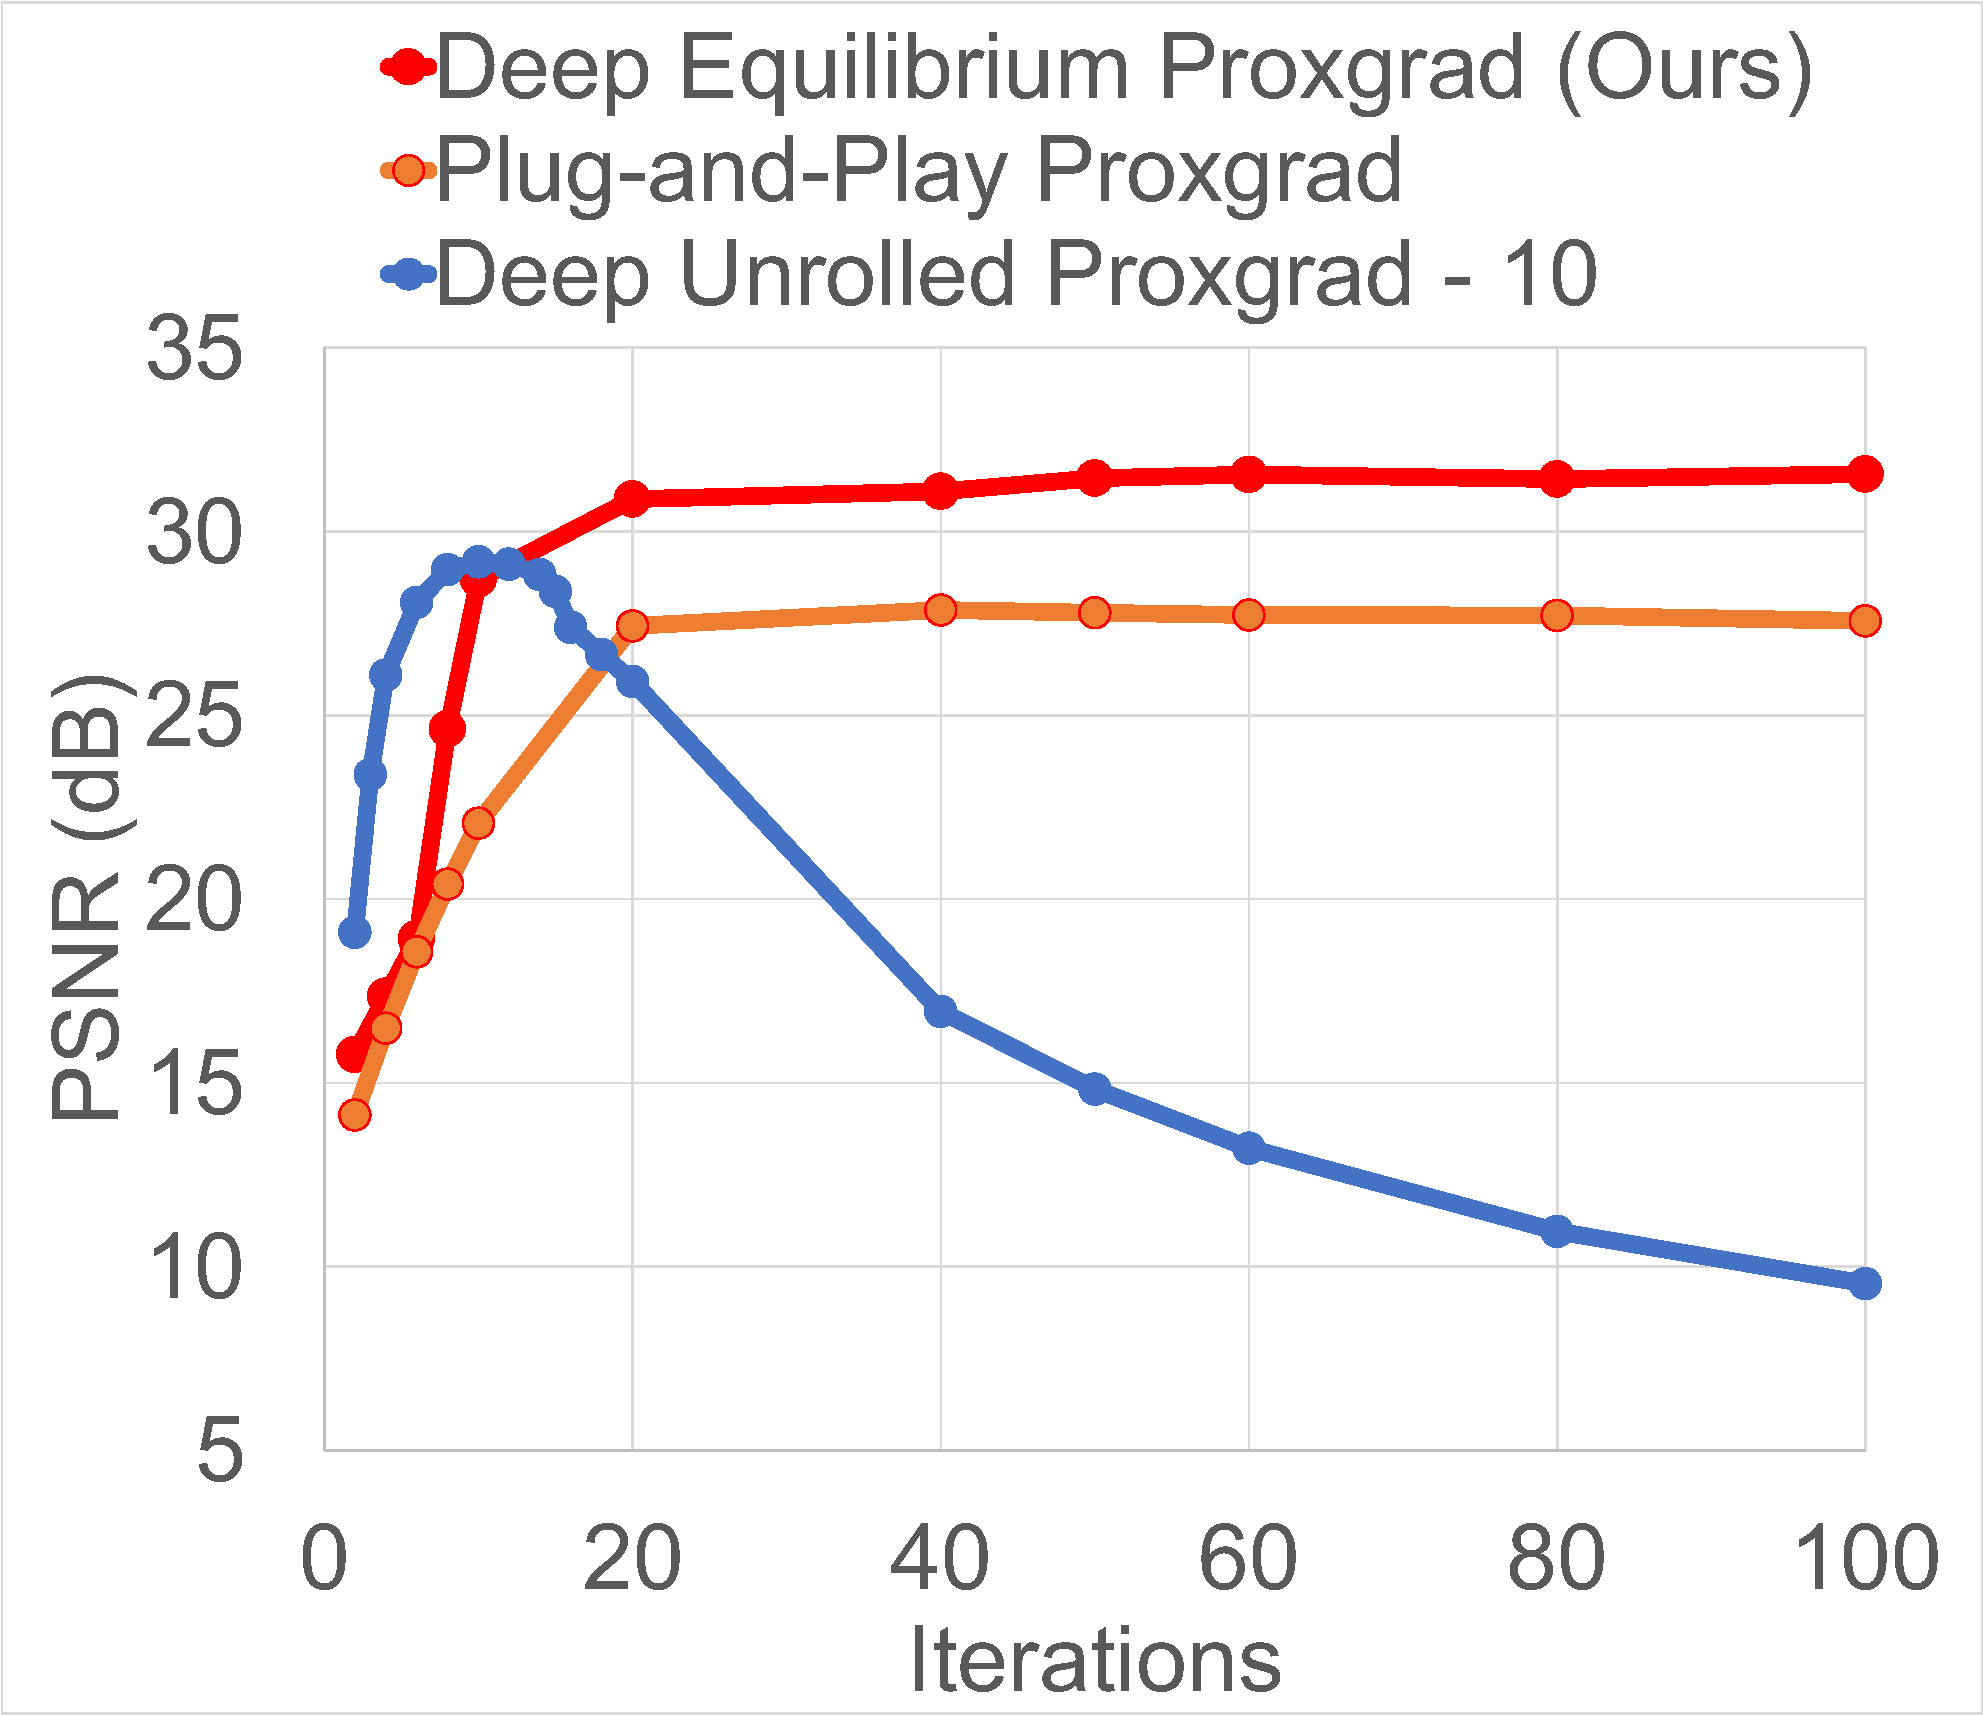
\includegraphics[width=0.6\textwidth]{deq/ResultsCS}
        \caption{Deep unrolling is primarily effective at the specific depth for which it was trained. DEMs achieve stable, higher PSNR across a broad infinite horizon \citep{gilton2021deep}.}
    \end{figure}
\end{frame}

\begin{frame}{Visual Comparison: 8x Accelerated MRI}
    \begin{figure}[htpb]
        \centering
        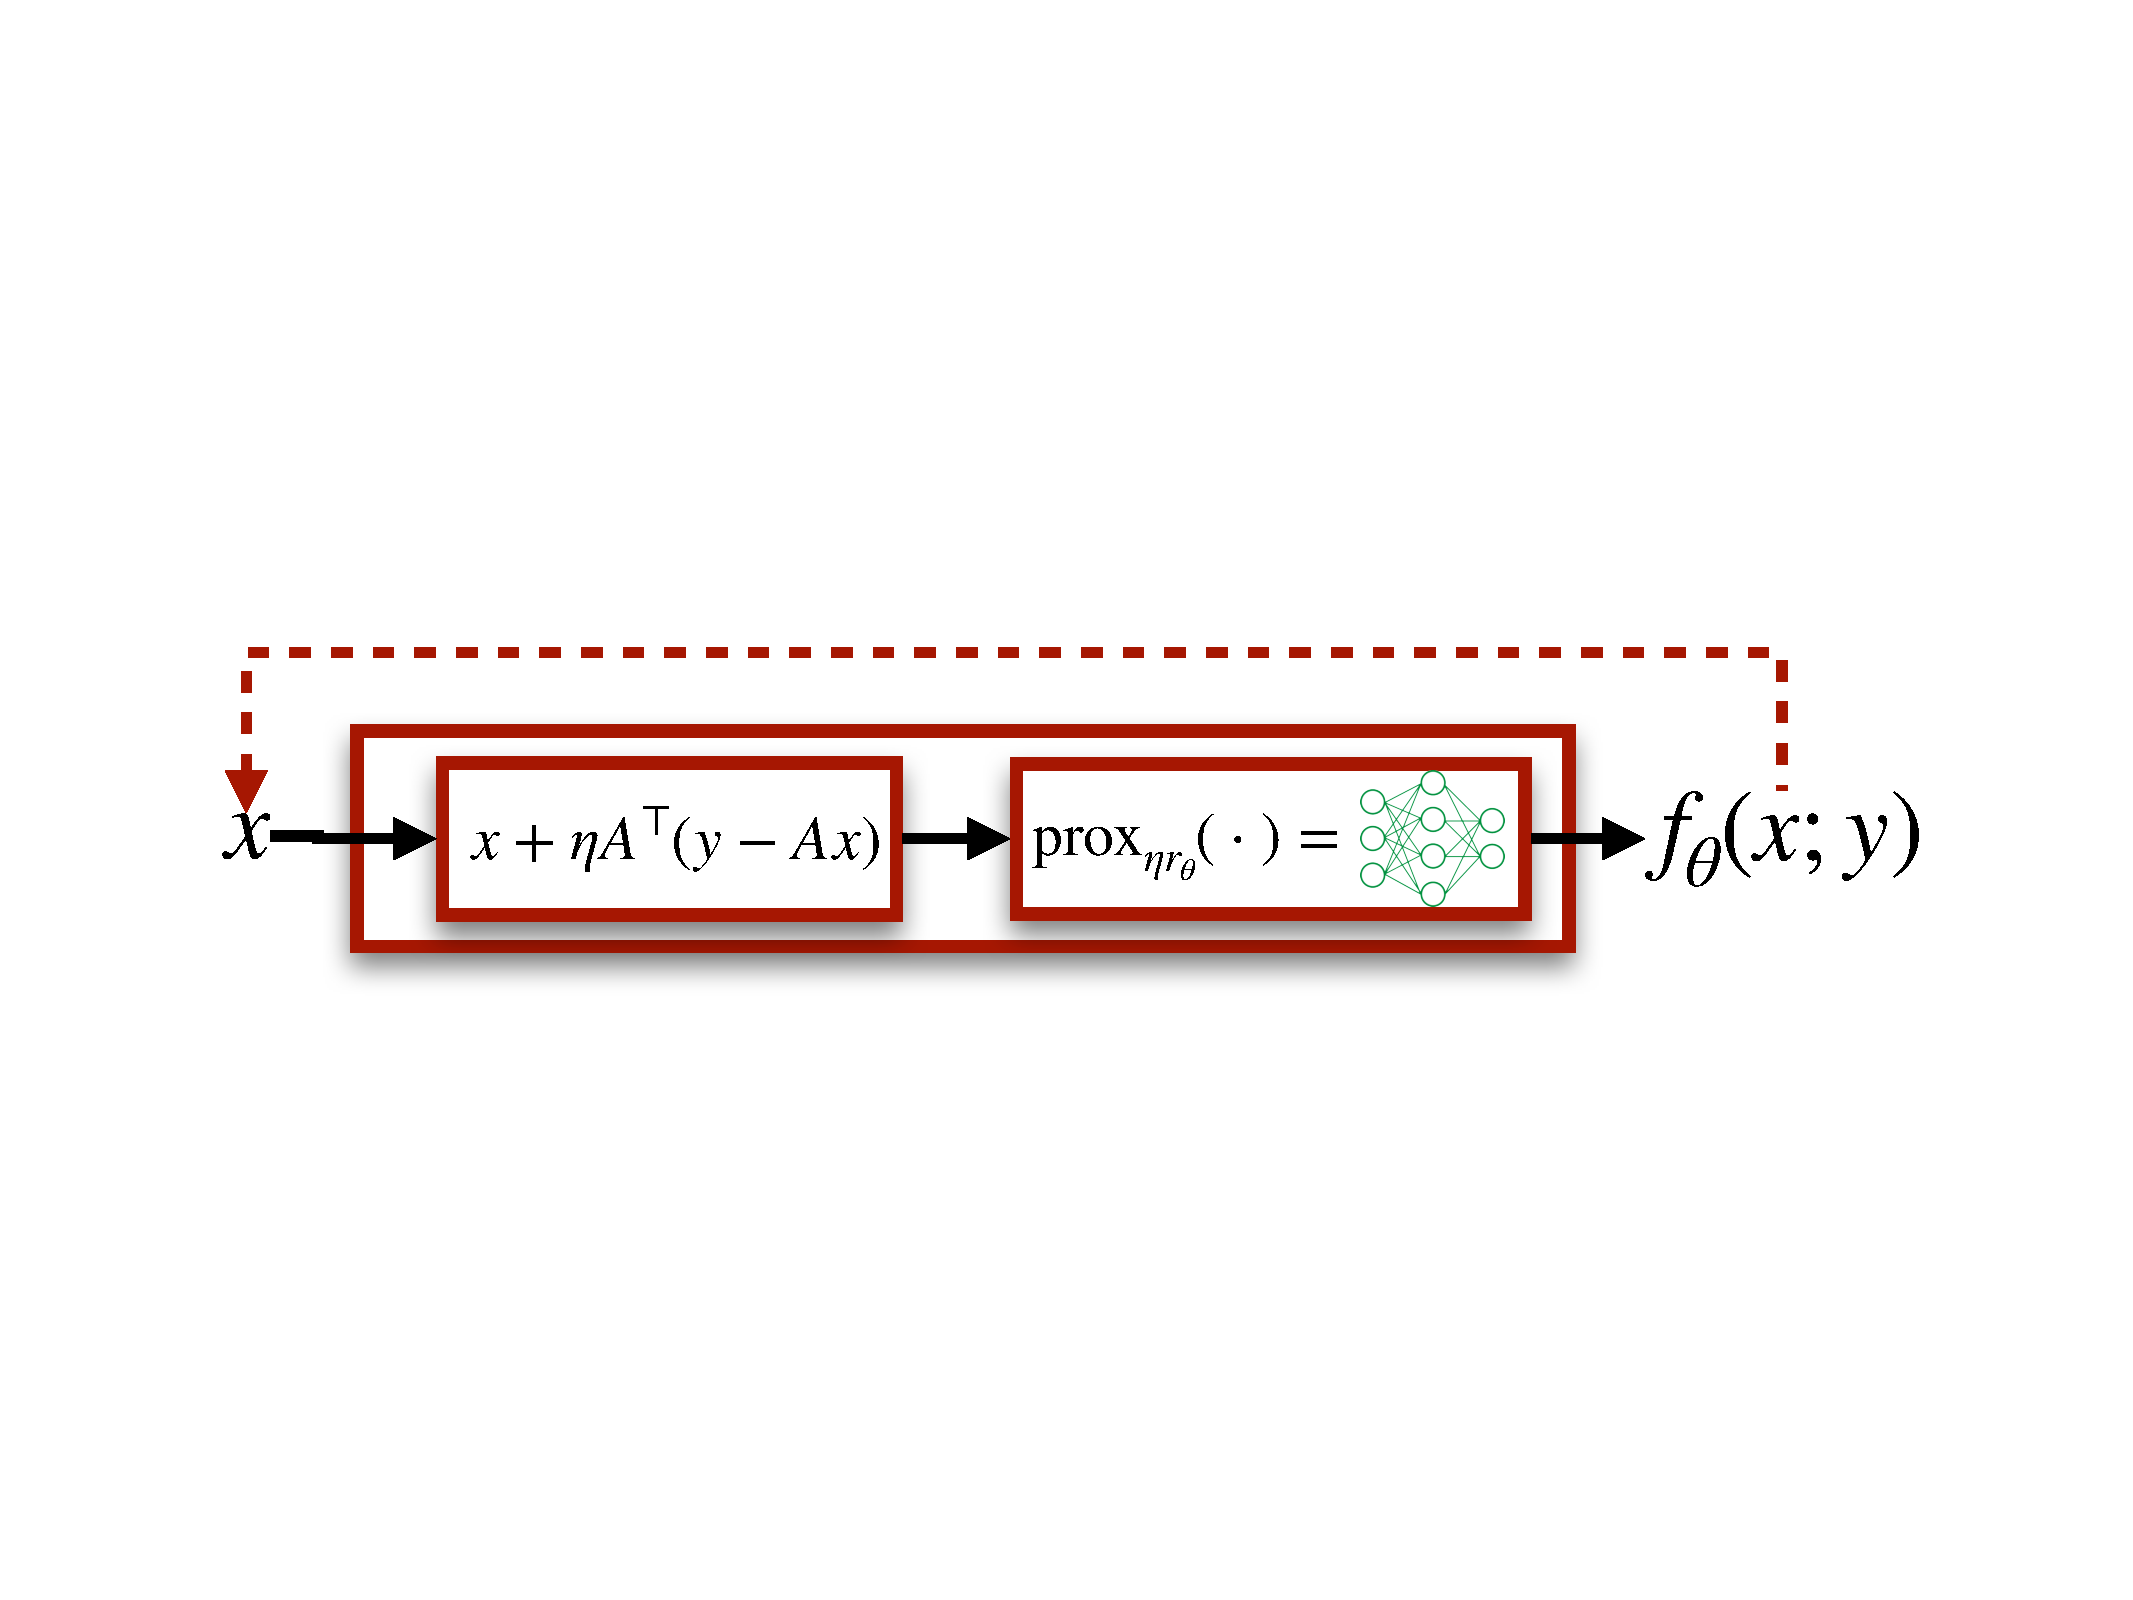
\includegraphics[width=0.9\textwidth]{deq/DEProx}
        \caption{Architecture of the Deep Equilibrium Proximal Gradient Descent (DE-PROX) model \citep{gilton2021deep}.}
    \end{figure}
\end{frame}

\begin{frame}{Closing the Loop: DEQs vs. Bilevel Learning}
    On Tuesday, we introduced \textbf{Bilevel Learning} to optimise regularisation hyperparameters by solving a lower-level variational problem. 
    
    \vspace{0.5em}
    As verified in \citet{riccio2022regularization}, Bilevel Learning can be seen as a subclass of Deep Equilibrium Models.
    
    \begin{itemize}
        \item \textbf{Bilevel Models:} The equilibrium map is structurally constrained to be the gradient of an explicit potential energy function (ensuring theoretical interpretability).
        \item \textbf{DEQs:} Learn an unconstrained, non-conservative map, offering more flexible fixed-point dynamics.
    \end{itemize}
\end{frame}

%================================================================%
\section{Summary}
%================================================================%

\begin{frame}{Summary of this Week}
    Over the course of this module, we have fundamentally dismantled the notion of Deep Learning as a rigid, black-box mapping:
    
    \begin{enumerate}
        \item \textbf{Algorithm Unrolling:} Embedding mathematical physics into explicit architectures.
        \item \textbf{Modular Models:} Using PnP, Score Matching, and Diffusion to decouple learned generative priors from deterministic inversion operators.
        \item \textbf{Continuous Dynamics:} Treating depth as continuous time, framing learning as optimal control, and leveraging symplectic integrators.
        \item \textbf{Implicit DEQs:} Abandoning explicit layers entirely to train infinite-depth networks with $\mathcal{O}(1)$ memory via root-finding and implicit differentiation.
    \end{enumerate}
\end{frame}

\begin{frame}[allowframebreaks]{References}
    \bibliographystyle{plainnat}
    \bibliography{references}
\end{frame}

\end{document}